\clearpage

\subsection{Architettura di dettaglio - Classi del sistema Monolith}
Nel caso dei componenti React la descrizione dello schema dell'oggetto props passato come argomento al costruttore è fornita indirettamente dall'elenco delle props.
\subsubsection{Check}
\textbf{Componente:}  Monolith::checks\\
   \FloatBarrier
   \begin{figure}[ht]
   \centering
   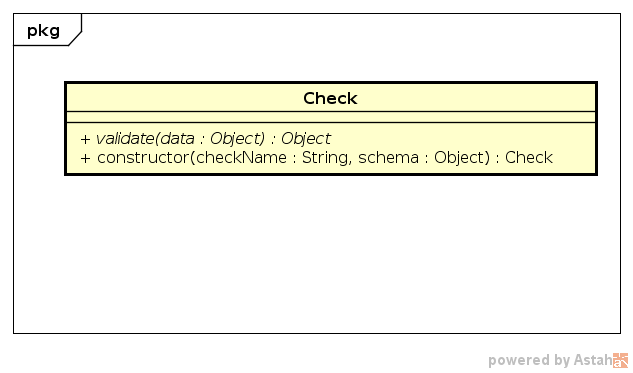
\includegraphics[width=0.6\textwidth]{img/single-Check.png}
   \caption{{Diagramma per Check in checks}}
\end{figure}
\FloatBarrier
\textbf{Descrizione}\\
Classe che rappresenta i controlli da eseguire lato server sull'input dell'utente. 
\begin{itemize}
\item +constructor(checkName: String, schema: Object) \\
Il costruttore riceve il nome con cui verrà registrato il controllo da eseguire e la descrizione dello schema dei dati. Il secondo argomento viene utilizzato per inizializzare un oggetto SimpleSchema.
\item +validate(dataObj:Object):boolean \\
Viene controllato che l'oggetto fornito come argomento corrisponda allo schema.
\end{itemize}
\emph{dataObj} è un oggetto Javascript formato da soli attributi (non funzioni) che viene validato rispetto allo schema registrato nel check del tipo corrispondente. Per ciascuna istanza della classe check si può trovare lo schema dei dati in \S 3.6

\emph{schema} rappresenta lo schema che devono avere i dati relativi alla bolla per poter essere inseriti nel database. Le definizioni degli schemi seguono la notazione SimpleSchema descritta in \S 3.6 


\textbf{Applicazioni}\\
Prima di ogni inserimento sul database i dati vengono verificati utilizzando questa classe. 


\clearpage

\subsubsection{CheckHandler}
\textbf{Componente:}  Monolith::checks\\
   \FloatBarrier
   \begin{figure}[ht]
   \centering
   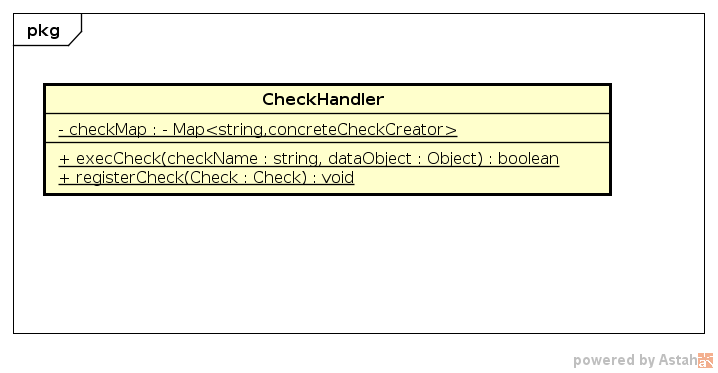
\includegraphics[width=0.6\textwidth]{img/single-CheckHandler.png}
   \caption{{Diagramma per CheckHandler in checks}}
\end{figure}
\FloatBarrier
\textbf{Descrizione}\\
Classe che contiene una mappa statica che associa i controlli (classe check) alle stringhe che li descrivono. Tutti i metodi sono statici. Si tratta di un modo per rappresentare nel formalismo UML quello che in JavaScript è un oggetto globale.
\begin{itemize}
\item +registerCheck(check: Check) \\
Inserisce un check nella mappa
\item +execCheck(checkName:String, dataObj: Object):boolean \\
Esegue il check con il nome checkName sull'oggetto dataObj e ritorna un booleano che descrive la conformità dei dati. In caso il check non sia presente nella mappa allora viene lanciato un errore.
\end{itemize}
\emph{dataObj} è un oggetto Javascript formato da soli attributi (non funzioni) che viene validato rispetto allo schema registrato nel check del tipo corrispondente. Per ciascuna istanza della classe check si può trovare lo schema dei dati in \S 3.6

\emph{L'utilizzo di oggetti globali non costituisce una soluzione ideale. Per la motivazione si veda \S 3.7} 


\textbf{Applicazioni}\\
Viene utilizzato per eseguire i controlli sull'input lato server 


\clearpage

\subsubsection{BubbleDatabase}
\textbf{Componente:}  Monolith::Database\\
   \FloatBarrier
   \begin{figure}[ht]
   \centering
   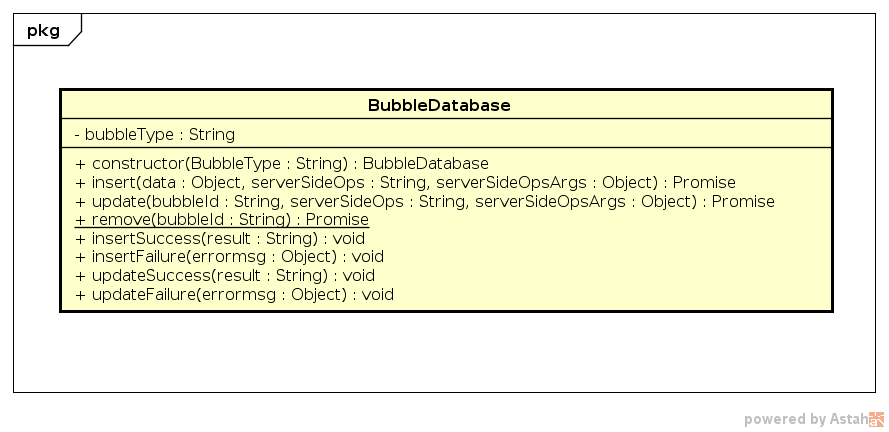
\includegraphics[width=0.6\textwidth]{img/single-BubbleDatabase.png}
   \caption{{Diagramma per BubbleDatabase in Database}}
\end{figure}
\FloatBarrier
\textbf{Descrizione}\\
Classe che fornisce un'interfaccia per utilizzare il database lato client. 
\\
Il costruttore chiede una stringa corrispondente al nome della bolla. Per ogni bolla si dovrà istanziare BubbleDatabase con il nome corrispondente.
\\
Ciascuno dei seguenti metodi ritorna una promise:
\begin{itemize} 
\item +insert(data: Object, serverSideOps, serverSideOpsArg) \\
Richiama il Meteor.Method insertBubble fornendo automaticamente alcuni parametri necessari e specificando la funzione lato server da eseguire sul database. data è un oggetto che contiene i dati da inserire nel database e la sua struttura dipende dai vari tipi di bolla.

La descrizione degli schemi realizzati da Obelix è in \S 3.6.

\item +update(bubbleId, serverSideOps, serverSideOpsArgs) \\
Richiama il Meteor.Method updateBubble specificando la funzione lato server da eseguire sul database.
\item +remove(bubbleId) \\
Metodo che richiama il Meteor.method per rimuovere la bolla con l'id passato come argomento
\end{itemize}
I restanti metodi (insertSuccess, insertFailure, updateSuccess, updateFailure) vengono invocati automaticamente al successo o al fallimento di una delle operazioni sopra descritte e semplicemente stampano un messaggio sulla console. In caso di necessità possono essere ridefiniti derivando la classe.

\emph{serverSideOps} è il nome di un Meteor.Method che può essere eseguito sui dati inviati prima dell'inserimento effettivo sul database. Nel caso dell'update è l'unico modo per effettuare modifiche. 

\emph{serverSideOpsArgs} è l'argomento di serverSideOps e può essere di qualunque tipo a seconda del caso. 


\textbf{Applicazioni}\\
Ogni tipo di bolla deve istanziare questa classe. Per ciascuna bolla, quindi, viene utilizzata come interfaccia alle operazioni di database. Assicura l'utilizzo corretto dei Meteor.Method da utilizzare per assicurare il corretto funzionamento di Monolith. 


\clearpage

\subsubsection{SideArea2}
\textbf{Componente:}  Monolith::SideAreas::ReceiveOperations\\
   \FloatBarrier
   \begin{figure}[ht]
   \centering
   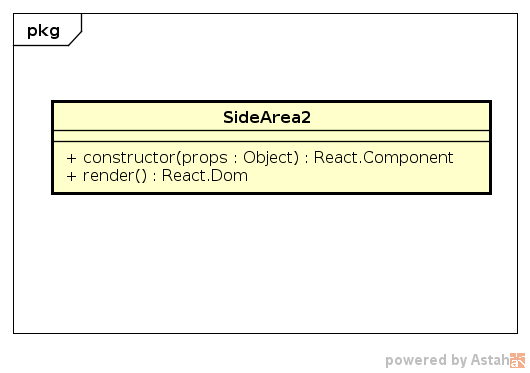
\includegraphics[width=0.6\textwidth]{img/single-SideArea2.png}
   \caption{{Diagramma per SideArea2 in ReceiveOperations}}
\end{figure}
\FloatBarrier
\textbf{Descrizione}\\
Classe che rappresenta il componente React per la visualizzazione del contenuto della seconda area laterale.
Non viene esportata direttamente, al suo posto si esporta SideArea2Container. Questa è realizzata con createContainer di react-meteor-data (si veda sezione \S 2.16).
 \\
\textbf{Metodi:} 
\begin{itemize}

\item +constructor(props : Object) : React.Component 
\\
Costruttore della sottoclasse di React.Component in cui è necessario chiamare super (props) ed è possibile inizializzare lo stato per i dati soggetti a cambiamento.

\item +render() : React.DOM 
\\
Metodo che esamina this.props e this.state e restituisce un componente che funge da contenitore per la seconda area laterale.

\end{itemize}


\textbf{Props:} 
\begin{itemize}
\item bubbles: 
\\
Array di oggetti che rappresentano le bolle che verranno passate al SentBubbles

\end{itemize} 


\textbf{Applicazioni}\\
Viene utilizzata all'apertura della seconda area laterale per visualizzare dello storico delle bolle ricevute. 


\clearpage

\subsubsection{ReceivedBubble}
\textbf{Componente:}  Monolith::SideAreas::ReceiveOperations\\
   \FloatBarrier
   \begin{figure}[ht]
   \centering
   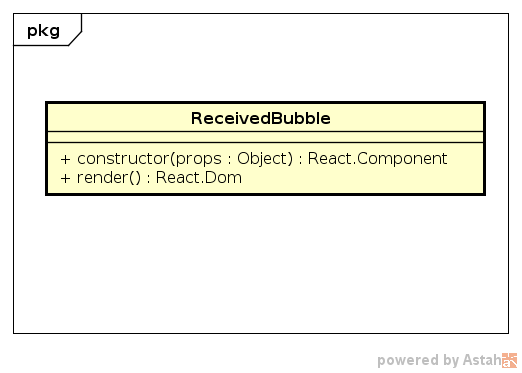
\includegraphics[width=0.6\textwidth]{img/single-ReceivedBubble.png}
   \caption{{Diagramma per ReceivedBubble in ReceiveOperations}}
\end{figure}
\FloatBarrier
\textbf{Descrizione}\\
Classe che rappresenta il componente React per la visualizzazione dello storico delle bolle ricevute. \\
\textbf{Metodi:} 
\begin{itemize}
\item +constructor(props : Object) : React.Component 
\\
Costruttore della sottoclasse di React.Component in cui è necessario chiamare super (props) ed è possibile inizializzare lo stato per i dati soggetti a cambiamento.
\item +render() : React.DOM 
\\
Metodo che esamina this.props e this.state e restituisce un singolo elemento React che può essere una rappresentazione di un componente DOM nativo o un altro componente composito.
\end{itemize}


\textbf{Props:} 
\begin{itemize}
\item bubbles: 
\\
Array di oggetti che rappresentano le bolle che verranno istanziate dal bubbleDiscriminator


\end{itemize} 


\textbf{Applicazioni}\\
Viene utilizzata dalla SideArea2 per la visualizzazione dello storico delle bolle ricevute. 


\clearpage

\subsubsection{SideArea1}
\textbf{Componente:}  Monolith::SideAreas::SendOperations\\
   \FloatBarrier
   \begin{figure}[ht]
   \centering
   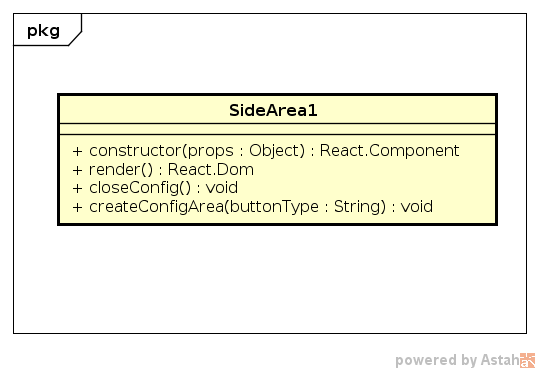
\includegraphics[width=0.6\textwidth]{img/single-SideArea1.png}
   \caption{{Diagramma per SideArea1 in SendOperations}}
\end{figure}
\FloatBarrier
\textbf{Descrizione}\\
Classe che rappresenta il componente React per la visualizzazione del contenuto della prima area laterale. \\
Non viene esportata direttamente, al suo posto si esporta SideArea1Container. Questa è realizzata con createContainer di react-meteor-data (si veda sezione \S 2.16).
 
\textbf{Metodi:}
\begin{itemize}

\item +constructor(props : Object) : React.Component 
\\
Costruttore della sottoclasse di React.Component in cui è necessario chiamare super (props) ed è possibile inizializzare lo stato per i dati soggetti a cambiamento.

\item +render() : React.DOM 
\\
Metodo che esamina this.props e this.state e restituisce un componente che funga da contenitore per la prima area laterale.

\end{itemize}


\textbf{Props:} 
\begin{itemize}
\item bubbles: 
\\
Array di oggetti che rappresentano le bolle che verranno passate al SentBubbles

\end{itemize} 


\textbf{Applicazioni}\\
Viene utilizzata all'apertura della prima area laterale per visualizzare il menù di creazione delle bolle e lo storico delle bolle inviate. 


\clearpage

\subsubsection{BubbleMenu}
\textbf{Componente:}  Monolith::SideAreas::SendOperations\\
   \FloatBarrier
   \begin{figure}[ht]
   \centering
   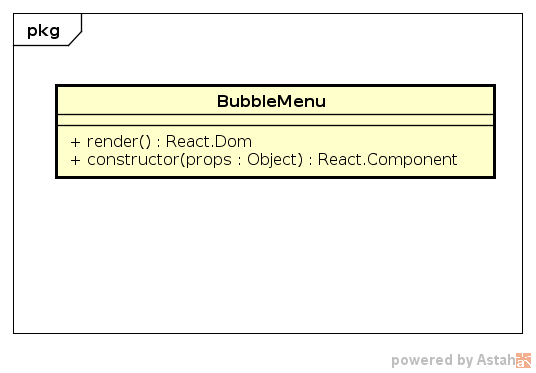
\includegraphics[width=0.6\textwidth]{img/single-BubbleMenu.png}
   \caption{{Diagramma per BubbleMenu in SendOperations}}
\end{figure}
\FloatBarrier
\textbf{Descrizione}\\
Classe che contiene i pulsanti che portano alla configurazione delle singole bolle.
\textbf{Metodi:} 
\begin{itemize}
\item +constructor(props : Object) : React.Component 
\\
Costruttore della sottoclasse di React.Component in cui è necessario chiamare super (props) ed è possibile inizializzare lo stato per i dati soggetti a cambiamento.
\item +render() : React.DOM 
\\
Metodo che esamina this.props e this.state e restituisce un singolo elemento React che può essere una rappresentazione di un componente DOM nativo o un altro componente composito.
\end{itemize}

\textbf{Props}:
\begin{itemize}
\item createConfigArea
\\
Metodo di SideArea1 che permette di inserire un componente React nell'area adibita al menu di configurazione. Viene passata ai bottoni.
\end{itemize} 


\textbf{Applicazioni}\\
Viene utilizzata dalla SideArea1 per la visualizzazione del menù contenente i pulsanti per la creazione delle bolle. 


\clearpage

\subsubsection{ConfigArea}
\textbf{Componente:}  Monolith::SideAreas::SendOperations\\
   \FloatBarrier
   \begin{figure}[ht]
   \centering
   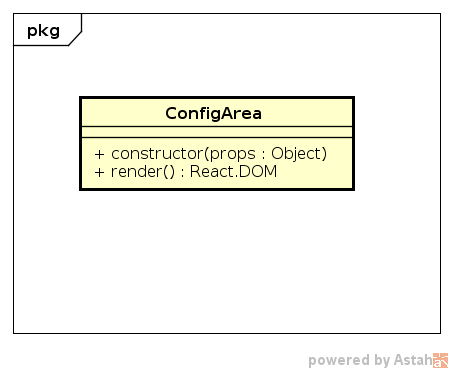
\includegraphics[width=0.6\textwidth]{img/single-ConfigArea.png}
   \caption{{Diagramma per ConfigArea in SendOperations}}
\end{figure}
\FloatBarrier
\textbf{Descrizione}\\
Componente React in cui la SideArea1 inserisce i componenti grafici di configurazione. Questi possono essere i menu di configurazione per le bolle o altri menu di impostazioni 


\textbf{Applicazioni}\\
Viene utilizzato da SideArea1 per mostrare componenti grafici a scomparsa 


\clearpage

\subsubsection{SentBubbles}
\textbf{Componente:}  Monolith::SideAreas::SendOperations\\
   \FloatBarrier
   \begin{figure}[ht]
   \centering
   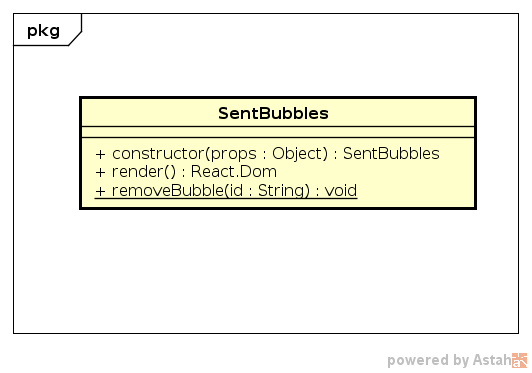
\includegraphics[width=0.6\textwidth]{img/single-SentBubble.png}
   \caption{{Diagramma per SentBubbles in SendOperations}}
\end{figure}
\FloatBarrier
\textbf{Descrizione}\\
Classe che rappresenta il componente React per la visualizzazione dello storico delle bolle inviate.

\textbf{Metodi:} 
\begin{itemize}

\item +constructor(props : Object) : React.Component 
\\
Costruttore della sottoclasse di React.Component in cui è necessario chiamare super (props) ed è possibile inizializzare lo stato per i dati soggetti a cambiamento.

\item +render() : React.DOM 
\\
Metodo che esamina this.props e this.state e restituisce un componente che raccolga lo storico delle bolle inviate.

\end{itemize}


\textbf{Props:} 
\begin{itemize}
\item bubbles: 
\\
Array di oggetti che rappresentano le bolle che verranno istanziate dal bubbleDiscriminator


\end{itemize} 


\textbf{Applicazioni}\\
Viene utilizzata dalla SideArea1 per la visualizzazione dello storico delle bolle inviate. 


\clearpage

\subsubsection{VerticalLayout}
\textbf{Componente:}  Monolith::UI::Layouts\\
   \FloatBarrier
   \begin{figure}[ht]
   \centering
   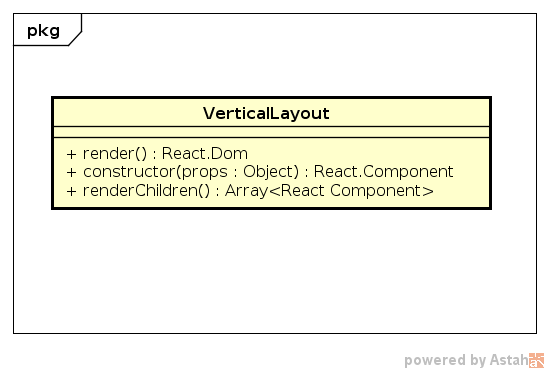
\includegraphics[width=0.6\textwidth]{img/single-VerticalLayout.png}
   \caption{{Diagramma per VerticalLayout in Layouts}}
\end{figure}
\FloatBarrier
\textbf{Descrizione}\\
Classe contenitore che dispone i componenti contenuti in verticale. \\
\textbf{Metodi:}
\begin{itemize}

\item +constructor(props : Object) : React.Component 
\\
Costruttore della sottoclasse di React.Component in cui è necessario chiamare super (props) ed è possibile inizializzare lo stato per i dati soggetti a cambiamento.

\item +render() : React.DOM 
\\
Metodo che esamina this.props e this.state e restituisce un contenitore di elementi che li dispone in verticale.

\item +countMyChildren() : int
\\
Metodo che ritorna un intero contente il numero di componenti figli, utilizzato per impostare la classe bootstrap corretta.

\end{itemize}

\textbf{Props:} 
\begin{itemize}
\item hide: 
\\
Booleano che provoca l'inserimento o meno di una classe HTML che nasconde il componente
\item classNames: 
\\
Array di stringhe che rappresentano classi HTML

\end{itemize} 


\textbf{Applicazioni}\\
Utilizzata per assegnare l'attributo className bootstrap a tutti i componenti figli, in modo che vengano visualizzati allineati in verticale con la dimensione adeguata. 


\clearpage

\subsubsection{ContainedElement}
\textbf{Componente:}  Monolith::UI::Layouts\\
   \FloatBarrier
   \begin{figure}[ht]
   \centering
   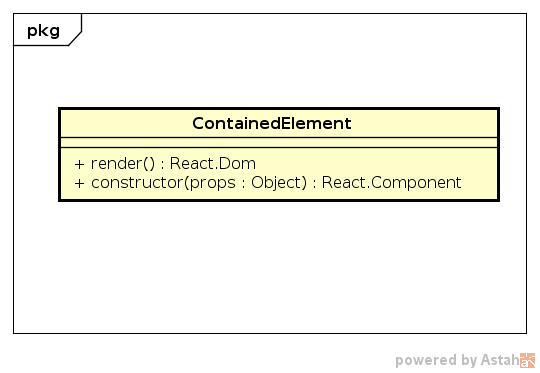
\includegraphics[width=0.6\textwidth]{img/single-ContainedElement.png}
   \caption{{Diagramma per ContainedElement in Layouts}}
\end{figure}
\FloatBarrier
\textbf{Descrizione}\\
Classe che rappresenta il layout di un contenitore generico. \\
\textbf{Metodi:} 
\begin{itemize}

\item +constructor(props : Object) : React.Component 
\\
Costruttore della sottoclasse di React.Component in cui è necessario chiamare super (props) ed è possibile inizializzare lo stato per i dati soggetti a cambiamento.

\item +render() : React.DOM 
\\
Metodo che esamina this.props e this.state e restituisce un elemento "div" contenenti i figli ed utilizzando lo stile CSS passato nella props "classNames".

\end{itemize}

\textbf{Props:} 
\begin{itemize}

\item classNames: 
\\
Array di stringhe che rappresentano classi HTML

\end{itemize} 


\textbf{Applicazioni}\\
Viene utilizzata dalle classi HorizontalLayout, VerticalLayout e ConditionalRendering per contenere un componente generico 


\clearpage

\subsubsection{HorizontalLayout}
\textbf{Componente:}  Monolith::UI::Layouts\\
   \FloatBarrier
   \begin{figure}[ht]
   \centering
   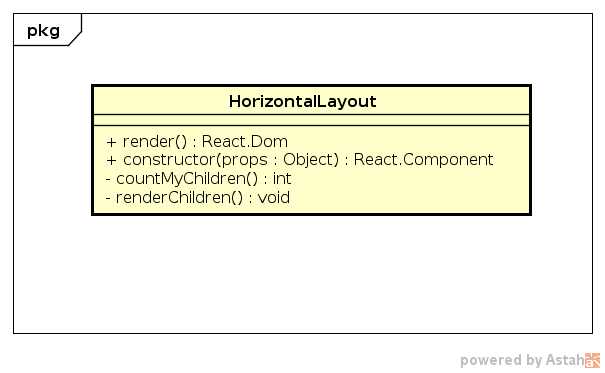
\includegraphics[width=0.6\textwidth]{img/single-HorizontalLayout.png}
   \caption{{Diagramma per HorizontalLayout in Layouts}}
\end{figure}
\FloatBarrier
\textbf{Descrizione}\\
Classe contenitore che dispone i componenti contenuti in orizzontale. \\
\textbf{Metodi:}
\begin{itemize}

\item +constructor(props : Object) : React.Component 
\\
Costruttore della sottoclasse di React.Component in cui è necessario chiamare super (props) ed è possibile inizializzare lo stato per i dati soggetti a cambiamento.

\item +render() : React.DOM 
\\
Metodo che esamina this.props e this.state e restituisce un contenitore di elementi che li dispone in orizzontale.

\item +countMyChildren() : int \\
Metodo che ritorna un intero contente il numero di componenti figli, utilizzato per impostare la classe bootstrap corretta.

\end{itemize}

\textbf{Props:} 
\begin{itemize}
\item hide: 
\\
Booleano che provoca l'inserimento o meno di una classe HTML che nasconde il componente
\item classNames: 
\\
Array di stringhe che rappresentano classi HTML

\end{itemize} 


\textbf{Applicazioni}\\
Utilizzata per assegnare l'attributo className bootstrap a tutti i componenti figli, in modo che vengano visualizzati allineati in orizzontale con la dimensione adeguata. 


\clearpage

\subsubsection{Image}
\textbf{Componente:}  Monolith::UI::SingleComponents\\
   \FloatBarrier
   \begin{figure}[ht]
   \centering
   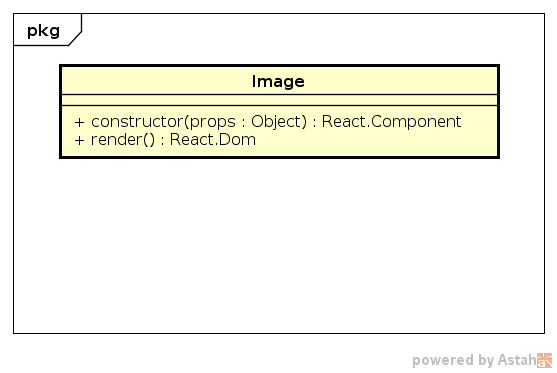
\includegraphics[width=0.6\textwidth]{img/single-Image.png}
   \caption{{Diagramma per Image in SingleComponents}}
\end{figure}
\FloatBarrier
\textbf{Descrizione}\\
Componente React che rappresenta un'immagine. \\
\textbf{Metodi:} 
\begin{itemize}
\item +constructor(props : Object) : React.Component 
\\
Costruttore della sottoclasse di React.Component in cui è necessario chiamare super (props) ed è possibile inizializzare lo stato per i dati soggetti a cambiamento.
\item +render() : React.DOM 
\\
Metodo che esamina this.props e this.state e restituisce un immagine con le proprietà datele.
\end{itemize}

\textbf{Props:} 
\begin{itemize}
\item id: 
\\
Codice di identificazione univoco
\item classes: 
\\
Array di stringhe che rappresentano classi HTML
\item src
\\
Come l'omonimo attributo HTML
\item alt
\\
Come l'omonimo attributo HTML
\item width
\\
Come l'omonimo attributo HTML
\item height
\\
Come l'omonimo attributo HTML

\end{itemize} 


\textbf{Applicazioni}\\
Viene utilizzato per rappresentare un immagine all'interno di una bolla. 


\clearpage

\subsubsection{ComboBox}
\textbf{Componente:}  Monolith::UI::SingleComponents\\
   \FloatBarrier
   \begin{figure}[ht]
   \centering
   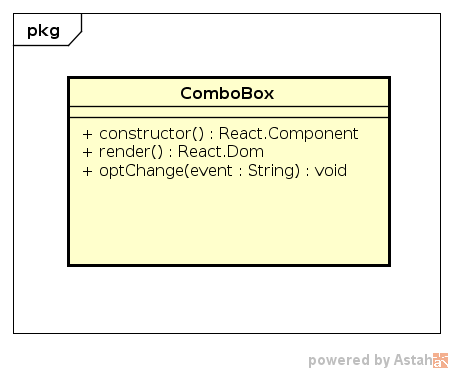
\includegraphics[width=0.6\textwidth]{img/single-ComboBox.png}
   \caption{{Diagramma per ComboBox in SingleComponents}}
\end{figure}
\FloatBarrier
\textbf{Descrizione}\\
Componente React che rappresenta un combobox. \\
\textbf{Metodi:} 
\begin{itemize}
\item +constructor(props : Object) : React.Component 
\\
Costruttore della sottoclasse di React.Component in cui è necessario chiamare super (props) ed è possibile inizializzare lo stato per i dati soggetti a cambiamento.

\item +optChange(event : String) : void  
\\
Comunica alla funzione "padre" l'opzione selezionata.

\item +render() : React.DOM 
\\
Metodo che esamina this.props e this.state e restituisce un singolo elemento combobox con le opzione passategli nelle props.

\end{itemize}

\textbf{Props:} 
\begin{itemize}
\item options: 
\\
Array di opzioni contenenti, per ciascuna di esse, una stringa.
\item classes: 
\\
Array di stringhe che rappresentano classi HTML
\item id:
\\
Stringa codice identificativo
\end{itemize} 


\textbf{Applicazioni}\\
Componente React rappresentante una combobox e costruibile passando un array contenente le varie opzioni nella props "options". 


\clearpage

\subsubsection{LineEdit}
\textbf{Componente:}  Monolith::UI::SingleComponents\\
   \FloatBarrier
   \begin{figure}[ht]
   \centering
   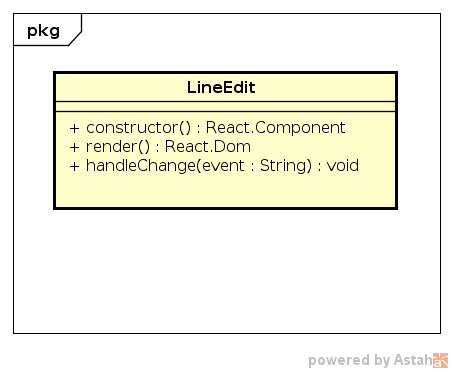
\includegraphics[width=0.6\textwidth]{img/single-LineEdit.png}
   \caption{{Diagramma per LineEdit in SingleComponents}}
\end{figure}
\FloatBarrier
\textbf{Descrizione}\\
Componente React che rappresenta un input di testo. \\
\textbf{Metodi:} 
\begin{itemize}
\item +constructor(props : Object) : React.Component 
\\
Costruttore della sottoclasse di React.Component in cui è necessario chiamare super (props) ed è possibile inizializzare lo stato per i dati soggetti a cambiamento.
\item +handleChange(event : String) : void  
\\
Comunica la stringa digitata al "padre". 
\item +render() : React.DOM 
\\
Metodo che esamina this.props e this.state e restituisce un singolo elemento React che rappresenta un input di testo.
\end{itemize}

\textbf{Props:} 
\begin{itemize}
\item id: 
\\
Codice di identificazione univoco
\item classes: 
\\
Array di stringhe che rappresentano classi HTML
\item value:
\\
Stringa che rappresenta il contenuto del campo di testo
\item placeholder
\\
Come l'omonimo attributo HTML

\end{itemize} 


\textbf{Applicazioni}\\
Viene utilizzato per costruire eventuali interfacce grafiche delle bolle. \\ 


\clearpage

\subsubsection{PushButton}
\textbf{Componente:}  Monolith::UI::SingleComponents\\
   \FloatBarrier
   \begin{figure}[ht]
   \centering
   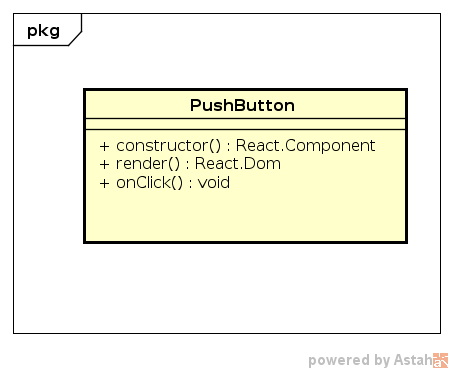
\includegraphics[width=0.6\textwidth]{img/single-PushButton.png}
   \caption{{Diagramma per PushButton in SingleComponents}}
\end{figure}
\FloatBarrier
\textbf{Descrizione}\\
Componente React che rappresenta un pulsante. \\
\textbf{Metodi:} 
\begin{itemize}
\item +constructor(props : Object) : React.Component 
\\
Costruttore della sottoclasse di React.Component in cui è necessario chiamare super (props) ed è possibile inizializzare lo stato per i dati soggetti a cambiamento.

\item +onClick(): void 
\\ 
Viene passato al "padre" l'ID del pulsante cliccato.

\item +render() : React.DOM 
\\
Metodo che esamina this.props e this.state e restituisce un singolo elemento React che rappresenta un pulsante eventualmente cliccabile.

\end{itemize}

\textbf{Props:} 
\begin{itemize}
\item id: 
\\
Identificativo univoco 
\item classes: 
\\
Array di stringhe che rappresentano classi HTML
\item buttonName
\\
Stringa che deve comparire nel bottone
\item dis
\\
Booleano per impostare la disabilitazione del pulsante
\item handleClick()
\\
Funzione che viene eseguita alla pressione del pulsante

\end{itemize} 


\textbf{Applicazioni}\\
Componente React che rappresenta un pulsante che può essere cliccabile (o meno) in base al valore della props "dis". \\ Questa può assumere valore \textit{true} o \textit{false}. 


\clearpage

\subsubsection{CheckButton}
\textbf{Componente:}  Monolith::UI::SingleComponents\\
   \FloatBarrier
   \begin{figure}[ht]
   \centering
   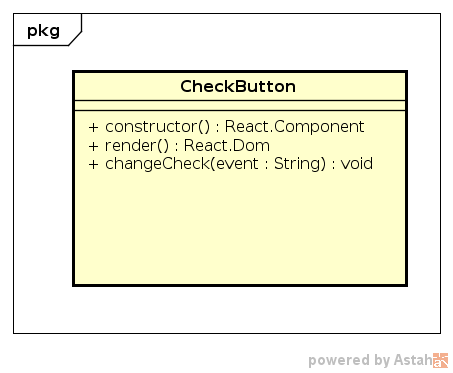
\includegraphics[width=0.6\textwidth]{img/single-CheckButton.png}
   \caption{{Diagramma per CheckButton in SingleComponents}}
\end{figure}
\FloatBarrier
\textbf{Descrizione}\\
Componente React che rappresenta un elemento di checkbox. \\
\textbf{Metodi:} 
\begin{itemize}

\item +constructor(props : Object) : React.Component 
\\
Costruttore della sottoclasse di React.Component in cui è necessario chiamare super (props) ed è possibile inizializzare lo stato per i dati soggetti a cambiamento.

\item +changeCheck(event : Object) : void  
\\
Comunica l’opzione selezionata tramite il metodo del genitore. event è l'oggetto generato dal DOM in seguito alla selezione di un elemento.

\item +render() : React.DOM 
\\
Metodo che esamina this.props e this.state e restituisce un singolo elemento React che può essere una rappresentazione di un componente DOM nativo o un altro componente composito.

\end{itemize}

\textbf{Props:} 
\begin{itemize}

\item classes: 
\\
Array di stringhe che rappresentano classi HTML
\item id:
\\
Identificativo univoco 
\item value:
\\
Stringa che deve essere associata al pulsante
\item getCheck():
\\
Funzione che restituisce un oggetto contenente l'id, il value e un booleano che rappresenta la pressione o meno del pulsante

\end{itemize} 


\textbf{Applicazioni}\\
Componente React che rappresenta un checkbox e contiene un metodo per comunicare al "padre" tutti i dati del oggetto quando questo viene cliccato. 


\clearpage

\subsubsection{ImageButton}
\textbf{Componente:}  Monolith::UI::SingleComponents\\
   \FloatBarrier
   \begin{figure}[ht]
   \centering
   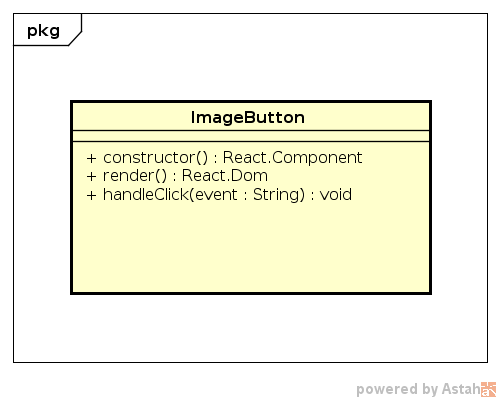
\includegraphics[width=0.6\textwidth]{img/single-ImageButton.png}
   \caption{{Diagramma per ImageButton in SingleComponents}}
\end{figure}
\FloatBarrier
\textbf{Descrizione}\\
Componente React che rappresenta un immagine che funge da pulsante. \\
\textbf{Metodi:} 
\begin{itemize}
\item +constructor(props : Object) : React.Component 
\\
Costruttore della sottoclasse di React.Component in cui è necessario chiamare super (props) ed è possibile inizializzare lo stato per i dati soggetti a cambiamento.
\item +handleClick() : void 
\\
Comunica l'Id dell'immagine cliccata al "padre". 
\item +render() : React.DOM 
\\
Metodo che esamina this.props e this.state e restituisce un singolo elemento React che rappresenta un'immagine cliccabile.
\end{itemize}

\textbf{Props:} 
\begin{itemize}
\item id: 
\\
Codice di identificazione univoco
\item classes: 
\\
Array di stringhe che rappresentano classi HTML
\item src
\\
Come l'omonimo attributo HTML
\item alt
\\
Come l'omonimo attributo HTML
\item width
\\
Come l'omonimo attributo HTML
\item height
\\
Come l'omonimo attributo HTML
\item onClick()
\\
Funzione da eseguire alla pressione del pulsante

\end{itemize} 


\textbf{Applicazioni}\\
Componente React che rappresenta un'immagine cliccabile.\\ 


\clearpage

\subsubsection{CheckBoxList}
\textbf{Componente:}  Monolith::UI::SingleComponents\\
   \FloatBarrier
   \begin{figure}[ht]
   \centering
   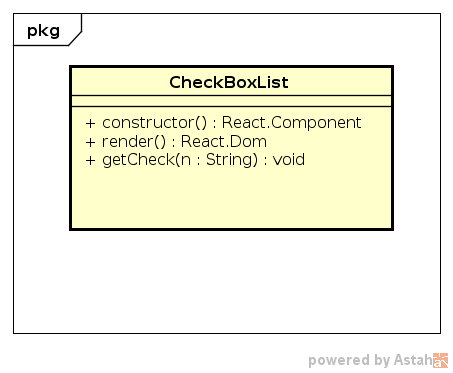
\includegraphics[width=0.6\textwidth]{img/single-CheckBoxList.png}
   \caption{{Diagramma per CheckBoxList in SingleComponents}}
\end{figure}
\FloatBarrier
\textbf{Descrizione}\\
Componente React che rappresenta una lista di CheckButton. \\
\textbf{Metodi:} 
\begin{itemize}
\item +constructor(props : Object) : React.Component 
\\
Costruttore della sottoclasse di React.Component in cui è necessario chiamare super (props) ed è possibile inizializzare lo stato per i dati soggetti a cambiamento.

\item +getCheck (n : Object) : void \\
Funzione che passa al "padre" i dati del CheckButton cliccato. 
n è l'oggetto ritorna da CheckButton

\item +render() : React.DOM 
\\
Metodo che esamina this.props e this.state e restituisce un singolo elemento React che può essere una rappresentazione di un componente DOM nativo o un altro componente composito.

\end{itemize}

\textbf{Props:} 
\begin{itemize}
\item options: 
\\
Passare un array di opzioni contenenti, per ciascuna di esse, un "id" ed un "value".
\item getCheck: 
\\
Passare una funzione che raccolga un oggetto di ritorno contenente i dati del CheckButton cliccato.

\end{itemize} 


\textbf{Applicazioni}\\
Componente React utile per costruire una lista di CheckButton passandogli un array di opzioni. 


\clearpage

\subsubsection{TextAreaButton}
\textbf{Componente:}  Monolith::UI::SingleComponents\\
   \FloatBarrier
   \begin{figure}[ht]
   \centering
   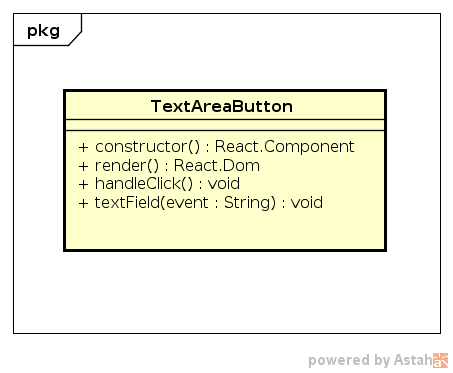
\includegraphics[width=0.6\textwidth]{img/single-TextAreaButton.png}
   \caption{{Diagramma per TextAreaButton in SingleComponents}}
\end{figure}
\FloatBarrier
\textbf{Descrizione}\\
Componente React che rappresenta un'area di testo con un pulsante. \\
\textbf{Metodi:} 
\begin{itemize}

\item +constructor(props : Object) : React.Component 
\\
Costruttore della sottoclasse di React.Component in cui è necessario chiamare super (props) ed è possibile inizializzare lo stato per i dati soggetti a cambiamento.

\item +textField(text : String) : void 
\\
Salva il testo scritto nella TextArea.

\item +handleClick(event : String) : void  
\\
Una volta cliccato il pulsante, passa al "padre" il testo raccolto. 

\item +render() : React.DOM 
\\
Metodo che esamina this.props e this.state e restituisce un componente React che unisce una TextArea ad un pulsate di invio.

\end{itemize}


\textbf{Props:} 
\begin{itemize}
\item classespb: 
\\
Array di classi HTML per il PushButton
\item classesta: 
\\
Array di classi HTML per la TextArea
\item idpb: 
\\
Identificativo univoco per il PushButton
\item idta: 
\\
Identificativo univoco per la TextArea
\item width: 
\\
Come l'attributo HTML omonimo per la TextArea
\item height: 
\\
Come l'attributo HTML omonimo per la TextArea
\item buttonName: 
\\
Stringa da rappresentare nel pulsante
\item getText(): 
\\
Funzione che restituisce il contenuto della TextArea



\end{itemize} 


\textbf{Applicazioni}\\
Componente React che può essere utilizzato per la costruzione delle interfacce di alcune bolle. 


\clearpage

\subsubsection{LineEditComboBox}
\textbf{Componente:}  Monolith::UI::SingleComponents\\
   \FloatBarrier
   \begin{figure}[ht]
   \centering
   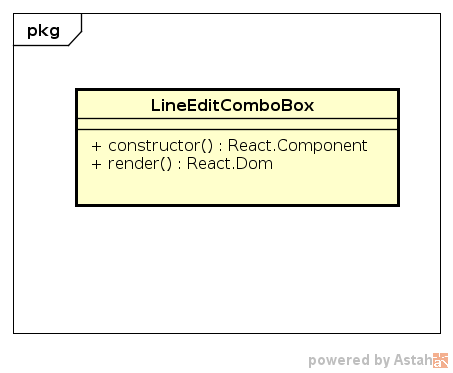
\includegraphics[width=0.6\textwidth]{img/single-LineEditComboBox.png}
   \caption{{Diagramma per LineEditComboBox in SingleComponents}}
\end{figure}
\FloatBarrier
\textbf{Descrizione}\\
Componente React che rappresenta una LineEdit con a fianco un ComboBox. \\
\textbf{Metodi:} 
\begin{itemize}

\item +constructor(props : Object) : React.Component 
\\
Costruttore della sottoclasse di React.Component in cui è necessario chiamare super (props) ed è possibile inizializzare lo stato per i dati soggetti a cambiamento.

\item +render() : React.DOM 
\\
Metodo che esamina this.props e this.state e restituisce un input di testo affiancato da una ComboBox.

\end{itemize}

\textbf{Props:} 
\begin{itemize}
\item idle: 
\\
Identificativo univoco per la LineEdit
\item idcb:
\\
Identificativo univoco per il ComboBox
\item classesle:
\\
Classe HTML per LineEdit
\item classescb: 
\\
Classe HTML per il ComboBox
\item comboUpdate()
\\
Funzione che riporta la modifica dello stato del ComboBox
\item options
\\
Array di stringhe per il ComboBox
\item textUpdate()
\\
Funzione che riporta la modifica dello stato del LineEdit
\end{itemize} 


\textbf{Applicazioni}\\
Componente React che unisce LineEdit e ComboBox.\\ 


\clearpage

\subsubsection{RadioButtonGroup}
\textbf{Componente:}  Monolith::UI::SingleComponents\\
   \FloatBarrier
   \begin{figure}[ht]
   \centering
   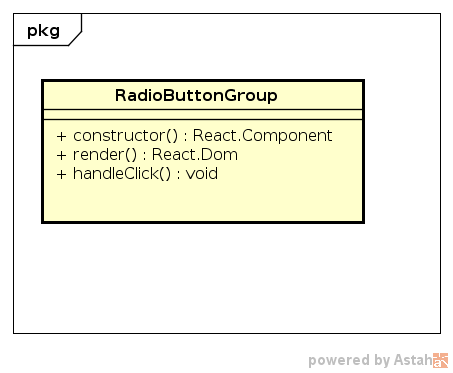
\includegraphics[width=0.6\textwidth]{img/single-RadioButtonGroup.png}
   \caption{{Diagramma per RadioButtonGroup in SingleComponents}}
\end{figure}
\FloatBarrier
\textbf{Descrizione}\\
Componente React che rappresenta un insieme di radio button tra cui è possibile scegliere tra opzioni mutualmente esclusive.\\

\textbf{Metodi:} 
\begin{itemize}
\item +constructor(props : Object) : React.Component 
\\
Costruttore della sottoclasse di React.Component in cui è necessario chiamare super (props) ed è possibile inizializzare lo stato per i dati soggetti a cambiamento.

\item +handleChange(event : Object): void 
\\
Viene passato al "padre" il valore selezionato. event è l'oggetto generato dal DOM alla scelta di un'opzione

\item +render() : React.DOM 
\\
Metodo che esamina this.props e this.state e restituisce un gruppo di RadioButton con le opzioni che sono state date.

\end{itemize}

\textbf{Props:} 
\begin{itemize}
\item options: 
\\
Array di opzioni contenenti, per ciascuna di esse, una stringa.
\item getValue(): 
\\
Funzione che viene eseguita alla selezione di un'opzione

\end{itemize} 


\textbf{Applicazioni}\\
Componente React che rappresenta un gruppo di RadioButton. \\ Le opzioni vengono passate con un array attraverso la props "options". 


\clearpage

\subsubsection{TextAreaComboBox}
\textbf{Componente:}  Monolith::UI::SingleComponents\\
   \FloatBarrier
   \begin{figure}[ht]
   \centering
   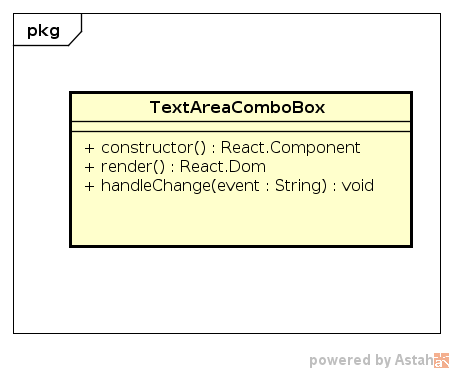
\includegraphics[width=0.6\textwidth]{img/single-TextAreaComboBox.png}
   \caption{{Diagramma per TextAreaComboBox in SingleComponents}}
\end{figure}
\FloatBarrier
\textbf{Descrizione}\\
Componente React che rappresenta una TextArea con a fianco un ComboBox \\\\
\textbf{Metodi:} 
\begin{itemize}

\item +constructor(props : Object) : React.Component 
\\
Costruttore della sottoclasse di React.Component in cui è necessario chiamare super (props) ed è possibile inizializzare lo stato per i dati soggetti a cambiamento.

\item +handleChange(event : String) : void  
\\ 
Comunica al "padre" il contenuto digitato nella textarea.

\item +render() : React.DOM 
\\
Metodo che esamina this.props e this.state e restituisce un componente React composto da una textArea ed un ComboBox.

\end{itemize}

\textbf{Props:} 
\begin{itemize}
\item classescb: 
\\
Array di classi HTML per il ComboBox
\item classestx: 
\\
Array di classi HTML per la TextArea
\item idcb: 
\\
Identificativo univoco per il ComboBox
\item idtx: 
\\
Identificativo univoco per la TextArea
\item width: 
\\
Come l'attributo HTML omonimo per la TextArea
\item height: 
\\
Come l'attributo HTML omonimo per la TextArea
\item options: 
\\
Array di opzioni per il ComboBox
\item textUpdate(): 
\\
Funzione che restituisce il contenuto della TextArea
\item comboUpdate():
\\
Funzione che restituisce il valore selezionato nel ComboBox



\end{itemize} 


\textbf{Applicazioni}\\
Componente React che può essere utilizzato per la costruzione delle interfacce di alcune bolle. 


\clearpage

\subsubsection{LineEditPushButton}
\textbf{Componente:}  Monolith::UI::SingleComponents\\
   \FloatBarrier
   \begin{figure}[ht]
   \centering
   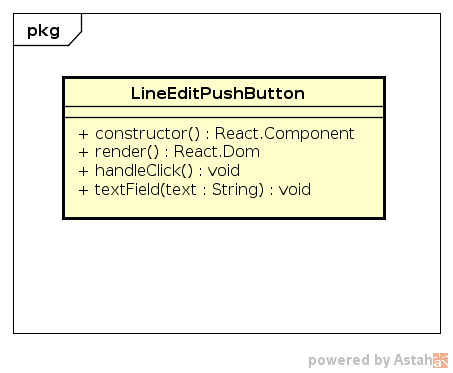
\includegraphics[width=0.6\textwidth]{img/single-LineEditPushButton.png}
   \caption{{Diagramma per LineEditPushButton in SingleComponents}}
\end{figure}
\FloatBarrier
\textbf{Descrizione}\\
Componente React che rappresenta un campo di inserimento testo affiancato ad un pulsante. \\
\textbf{Metodi:} 
\begin{itemize}

\item +constructor(props : Object) : React.Component 
\\
Costruttore della sottoclasse di React.Component in cui è necessario chiamare super (props) ed è possibile inizializzare lo stato per i dati soggetti a cambiamento.

\item +handleClick() : void  
\\
Passa al "padre" il testo contenuto nel LineEdit.

\item ++textField() : void  
\\
Salva nello state il testo presente nel LineEdit.

\item +render() : React.DOM 
\\
Metodo che esamina this.props e this.state e restituisce un componente React composto da un input di testo ed un pulsante di invio.

\end{itemize}

\textbf{Props:} 
\begin{itemize}
\item classesle: 
\\
classi HTML per il LineEdit
\item classespb: 
\\
classi HTML per il PushButton
\item idle
\\
Identificativo univoco per LineEdit
\item idpb
\\
Identificativo univoco per PushButton
\item buttonName
\\
testo da mostrare nel bottone
\item getText()
\\
Funzione che riporta il cambiamento di stato del LineEdit

\end{itemize} 


\textbf{Applicazioni}\\
Viene utilizzato per costruire alcune interfacce grafiche delle bolle. 


\clearpage

\subsubsection{AbsBubble}
\textbf{Componente:}  Monolith::UI::uiConstruction\\
   \FloatBarrier
   \begin{figure}[ht]
   \centering
   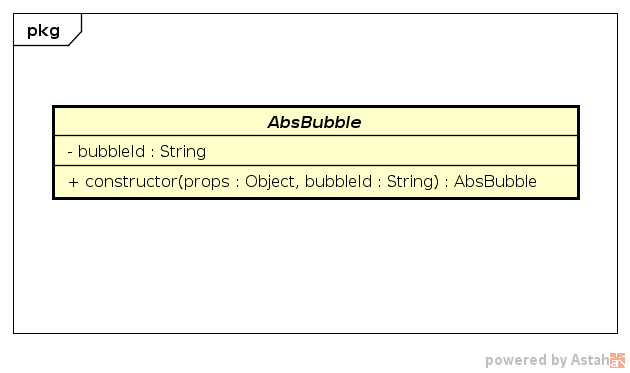
\includegraphics[width=0.6\textwidth]{img/single-AbsBubble.png}
   \caption{{Diagramma per AbsBubble in uiConstruction}}
\end{figure}
\FloatBarrier
\textbf{Descrizione}\\
Classe base astratta per le interfacce grafiche delle singole bolle. 


\textbf{Applicazioni}\\
Viene utilizzata come classe base da cui derivare le interfacce grafiche delle bolle. 


\clearpage

\subsubsection{AbsButton}
\textbf{Componente:}  Monolith::UI::uiConstruction\\
   \FloatBarrier
   \begin{figure}[ht]
   \centering
   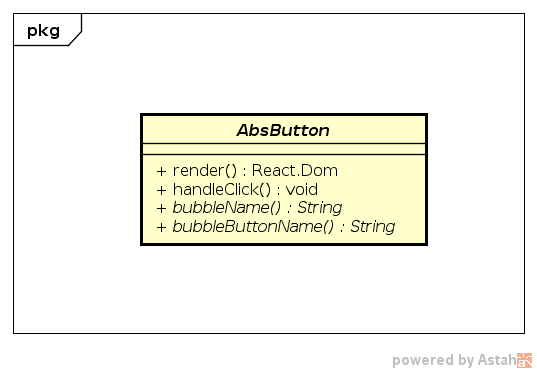
\includegraphics[width=0.6\textwidth]{img/single-AbsButton.png}
   \caption{{Diagramma per AbsButton in uiConstruction}}
\end{figure}
\FloatBarrier
\textbf{Descrizione}\\
Classe base dei pulsanti del menu di creazione delle nuove bolle. La classe base contiene molto codice e chiede classi derivate relativamente semplici. Viene usato il template pattern per parametrizzare gli aspetti che differiscono tra le classi derivate.
I seguenti metodi sono astratti puri:
\begin{itemize}
\item +bubbleName(): String \\
Nelle classi derivate ritorna il nome della bolla necessario per usare BubbleDiscriminator
\item +bubbleButtonName(): String \\
Nelle classi derivate ritorna il testo che deve comparire nel pulsante
\item +secondAreaName(): String \\
Nelle classi derivate ritorna il nome del componente React che deve essere inserito alla pressione del secondo pulsante. \\'E necessario per usare BubbleDiscriminator
\end{itemize}
I seguenti metodi semplicemente eseguono le funzioni che vengono passate nelle props in risposta alla pressione dei pulsanti:
\begin{itemize}
\item +handleClick():void
\item +handleSecondButton():void
\end{itemize}
Il metodo render crea uno o due pulsanti a seconda che sia definito o meno il testo da inserire nel secondo pulsante nelle props.

\textbf{Props:} 
\begin{itemize}
\item onClick(): 
\\
Funzione da eseguire alla pressione del secondo bottone 
\item id: 
\\
Stringa codice d'identificazione
\item secondButtonName
\\
Stringa che contiene il testo da visualizzare nel secondo bottone
\item classes
\\
Elenco di classi HTML
\end{itemize} 


\textbf{Applicazioni}\\
Classe base da cui derivare per ottenere i pulsanti del menu di creazione di di nuove bolle 


\clearpage

\subsubsection{bubbleCreator}
\textbf{Componente:}  Monolith::UI::uiConstruction\\
   \FloatBarrier
   \begin{figure}[ht]
   \centering
   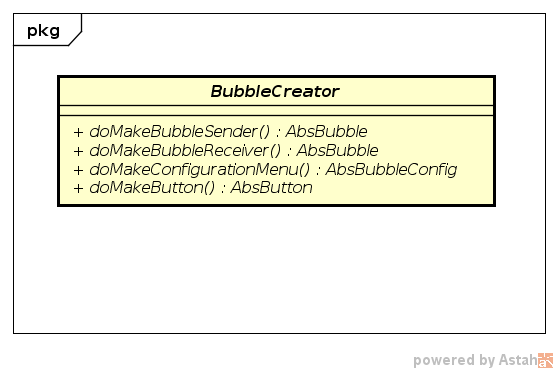
\includegraphics[width=0.6\textwidth]{img/single-bubbleCreator.png}
   \caption{{Diagramma per bubbleCreator in uiConstruction}}
\end{figure}
\FloatBarrier
\textbf{Descrizione}\\
Classe base astratta da cui poter derivare le classi concrete che si occupano della creazione delle istanze  di componenti grafici  \\ 
\textbf{Metodi:}
\begin{itemize}
\item +doMakeBubbleSender() : ConcreteBubble 
\\
Ritorna il componente React per visualizzare una bolla inviata.
\item +doMakeBubbleReceiver() : ConcreteBubble 
\\
Ritorna il componente React per visualizzare una bolla ricevuta.
\item +doMakeConfigurationMenu() : ConcreteBubbleConfig 
\\
Ritorna il componente React per visualizzare il menù di creazione di una bolla da inviare.
\item +doMakeButton() : ConcreteBubbleCreationButton 
\\
Ritorna il componente React per visualizzare il bottone di creazione del menù di configurazione di una bolla da inviare.

\end{itemize} 


\textbf{Applicazioni}\\
Interfaccia che viene utilizzata come rappresentazione di concreteBubbleCreator. 


\clearpage

\subsubsection{AbsBubbleConfig}
\textbf{Componente:}  Monolith::UI::uiConstruction\\
   \FloatBarrier
   \begin{figure}[ht]
   \centering
   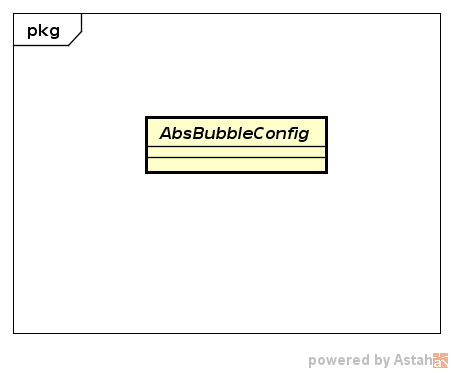
\includegraphics[width=0.6\textwidth]{img/single-AbsBubbleConfig.png}
   \caption{{Diagramma per AbsBubbleConfig in uiConstruction}}
\end{figure}
\FloatBarrier
\textbf{Descrizione}\\
Classe Astratta (interfaccia) per i menù di configurazione delle singole bolle. 


\textbf{Applicazioni}\\
Classe base da cui derivare per costruire i menù di configurazione delle bolle. 


\clearpage

\subsubsection{bubbleDiscriminator}
\textbf{Componente:}  Monolith::UI::uiConstruction\\
   \FloatBarrier
   \begin{figure}[ht]
   \centering
   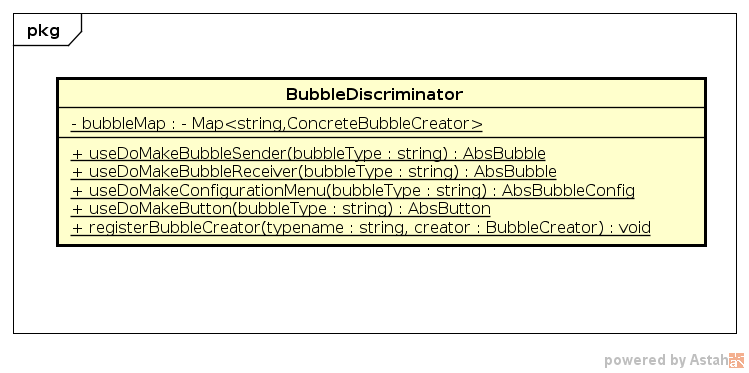
\includegraphics[width=0.6\textwidth]{img/single-bubbleDiscriminator.png}
   \caption{{Diagramma per bubbleDiscriminator in uiConstruction}}
\end{figure}
\FloatBarrier
\textbf{Descrizione}\\
Classe che contiene i metodi che ritornano le funzionalità necessarie per la rappresentazione delle bolle. Tutti i metodi sono statici. Si tratta di un modo per rappresentare nel formalismo UML quello che in JavaScript è un oggetto globale.

\textbf{Attributi:}
\begin{itemize}
\item -bubbleMap : Map$<$string,concreteBubbleCreator$>$ 
\\
Struttura che mappa il nome di una bolla con l'istanza di concreteBubbleCreator per quella bolla.
\end{itemize}
\textbf{Metodi:} 
\begin{itemize}
\item +useDoMakeBubbleSender( bubbleType: string) : ConcreteBubble \\
Ritorna il componente React della stringa passata come parametro per visualizzare una bolla inviata.
\item +useDoMakeBubbleReceiver( bubbleType: string) : ConcreteBubble \\
Ritorna il componente React della stringa passata come parametro per visualizzare una bolla ricevuta.
\item +useDoMakeBubbleConfigurationMenu( bubbleType: string) : ConcreteBubbleConfig 
\\
Ritorna il componente React della stringa passata come parametro per visualizzare il menù di creazione di una bolla da inviare.
\item  +useDoMakeButton( bubbleType: string) : ConcreteBubbleCreationButton \\
Ritorna il componente React della stringa passata come parametro per visualizzare il bottone di creazione del menù di configurazione di una bolla da inviare.

\end{itemize}

\emph{L'utilizzo di oggetti globali non costituisce una soluzione ideale. Per la motivazione si veda \S 3.7} 


\textbf{Applicazioni}\\
Viene utilizzata quando si deve creare una nuova bolla, ritornando l'oggetto della bolla appena selezionata. 


\subsection{Architettura di dettaglio - Classi delle bolle demo}
Nel caso dei componenti React la descrizione dello schema dell'oggetto props passato come argomento al costruttore è fornita indirettamente dall'elenco delle props.
\subsubsection{CurrencyBubble}
\textbf{Componente:}  CurrencyBubble\\
   \FloatBarrier
   \begin{figure}[ht]
   \centering
   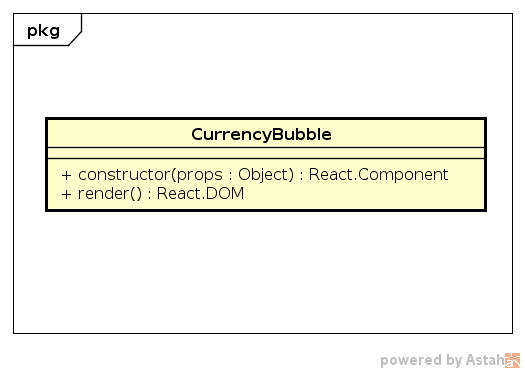
\includegraphics[width=0.6\textwidth]{img/single-CurrencyBubble.png}
   \caption{{Diagramma per CurrencyBubble in CurrencyBubble}}
\end{figure}
\FloatBarrier
\textbf{Descrizione}\\
Componente React che rappresenta l'interfaccia grafica di una CurrencyBubble
\\
\textbf{Metodi:} 
\begin{itemize}
\item +constructor(props : Object) : React.Component 
\\
Costruttore della sottoclasse di React.Component in cui è necessario chiamare super (props) ed è possibile inizializzare lo stato per i dati soggetti a cambiamento.

\item +render() : React.DOM 
\\
Metodo che esamina this.props e this.state e restituisce la CurrencyBubble a conversione avvenuta.

\end{itemize}

\textbf{Props:} 
\begin{itemize}
\item curr\_in: 
\\
Stringa che rappresenta la valuta in ingresso
\item curr\_out: 
\\
Stringa che rappresenta la valuta in uscita
\item value\_in
\\
Numero che rappresenta l'importo in ingresso
\item value\_out
\\
Numero che rappresenta l'importo in uscita

\end{itemize} 


\textbf{Applicazioni}\\
Viene utilizzata per rappresentare graficamente la bolla di conversione valuta. 


\clearpage

\subsubsection{CurrencyCreator}
\textbf{Componente:}  CurrencyBubble\\
   \FloatBarrier
   \begin{figure}[ht]
   \centering
   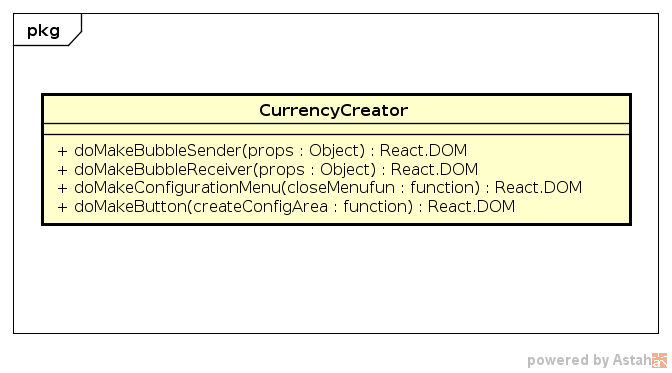
\includegraphics[width=0.6\textwidth]{img/single-CurrencyCreator.png}
   \caption{{Diagramma per CurrencyCreator in CurrencyBubble}}
\end{figure}
\FloatBarrier
\textbf{Descrizione}\\
Istanziazione concreta della classe Monolith::UI::uiConstruction::BubbleCreator che gestisce la creazione della singola istanza di bolla convertitore di valuta, della singola istanza di menù di configurazione della bolla e della singola istanza di pulsante tramite l'utilizzo della classe Monolith::UI::Bubbles::BubbleDiscriminator.
\\
\textbf{Metodi:} 
\begin{itemize}
\item +doMakeBubbleSender() : CurrencyBubble 
\\
Metodo che gestisce la creazione della bolla vista dal mittente.
\item +doMakeBubbleReceiver() : CurrencyBubble 
\\
Metodo che gestisce la creazione della bolla vista dal ricevente.
\item +doMakeConfigurationMenu() : CurrencyBubbleConfig 
\\
Metodo che gestisce la creazione dell'area di configurazione della bolla.
\item +doMakeButton() : CurrencyBubbleCreationButton 
\\
Metodo che gestisce la creazione della singola istanza di pulsante da inserire nel menu iniziale di creazione. Viene lasciata l'implementazione della super classe.
\end{itemize} 


\textbf{Applicazioni}\\
Viene utilizzata per gestire la creazione della singola istanza di bolla convertitore di valuta, della singola istanza di menù di configurazione della bolla e della singola istanza di pulsante. 


\clearpage

\subsubsection{CurrencyBubbleConfig}
\textbf{Componente:}  CurrencyBubble\\
   \FloatBarrier
   \begin{figure}[ht]
   \centering
   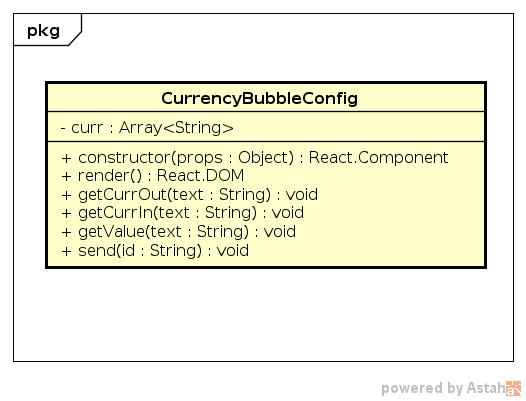
\includegraphics[width=0.6\textwidth]{img/single-CurrencyBubbleConfig.png}
   \caption{{Diagramma per CurrencyBubbleConfig in CurrencyBubble}}
\end{figure}
\FloatBarrier
\textbf{Descrizione}\\
Componente React che rappresenta il menù per la costruzione di una bolla di conversione valuta.
\\
\textbf{Metodi:} 
\begin{itemize}
\item +constructor(props : Object) : React.Component 
\\
Costruttore della sottoclasse di React.Component in cui è necessario chiamare super (props) ed è possibile inizializzare lo stato per i dati di conversione e per quelli soggetti a cambiamento.

\item +getCurrIn(text : String) : void 
\\
Salva la valuta di base.

\item +getCurrOut(text : String) : void 
\\
Salva la valuta di uscita.

\item +getValue(text : String) : void 
\\
Salva il valore iniziale di conversione.

\item +send() : void 
\\
Salva i dati raccolti e li passa al "padre".

\item +render() : React.DOM
\\
Metodo che esamina this.props e this.state, costruisce un array di opzioni modificabili e restituisce l'interfaccia grafica per il menù di creazione.
\end{itemize}

\textbf{Props:} 
\begin{itemize}
\item closeMenu(): 
\\
Funzione che permette al componente di cancellarsi. Viene utilizzato in caso di esito positivo dell'invio.


\end{itemize} 


\textbf{Applicazioni}\\
Viene utilizzato per rappresentare il menù di configurazione della bolla di conversione valuta. 


\clearpage

\subsubsection{CurrencyBubbleCreationButton}
\textbf{Componente:}  CurrencyBubble\\
   \FloatBarrier
   \begin{figure}[ht]
   \centering
   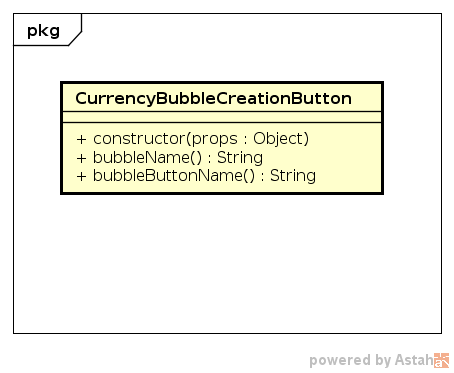
\includegraphics[width=0.6\textwidth]{img/single-CurrencyBubbleCreationButton.png}
   \caption{{Diagramma per CurrencyBubbleCreationButton in CurrencyBubble}}
\end{figure}
\FloatBarrier
\textbf{Descrizione}\\
Componente React che rappresenta il pulsante per creare una bolla di conversione valuta.
\\
\textbf{Metodi:} 
\begin{itemize}
\item +constructor(props : Object) : React.Component 
\\
Costruttore della sottoclasse di React.Component in cui è necessario chiamare super (props) ed è possibile inizializzare lo stato per i dati soggetti a cambiamento.

\item +bubbleButtonName() : String 
\\
Metodo che ritorna il nome presente sul pulsante.

\item +bubbleName() : String 
\\
Metodo che ritorna il nome identificativo della bolla .

\end{itemize}

\textbf{Props:} 
Non sono presenti props utilizzate direttamente. Vedere la superclasse AbsButton 


\textbf{Applicazioni}\\
Viene utilizzato per rappresentare il pulsante per la creazione di una bolla di conversione valuta. 


\clearpage

\subsubsection{AbsList}
\textbf{Componente:}  ListBubble\\
   \FloatBarrier
   \begin{figure}[ht]
   \centering
   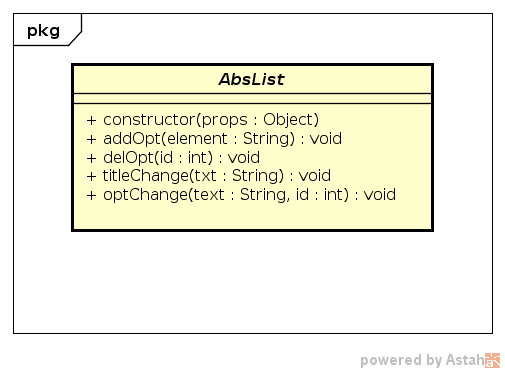
\includegraphics[width=0.6\textwidth]{img/single-AbsList.png}
   \caption{{Diagramma per AbsList in ListBubble}}
\end{figure}
\FloatBarrier
\textbf{Descrizione}\\
Componente React astratto che implementa alcuni metodi per la gestione di una lista al di fuori delle funzionalità grafiche che verranno implementate nelle derivate.
\\
\textbf{Metodi:} 
\begin{itemize}
\item +constructor(props : Object) : React.Component 
\\
Costruttore della sottoclasse di React.Component. La classe è astratta e dunque non può essere istanziata. Pertanto props dipende dalle specifiche classi derivate.

\item +addOpt(element : String) : void 
\\
Metodo che aggiunge un elemento alla lista.
\item +delOpt(id:int):void
\\
Metodo che cancella dalla lista l'elemento con l'id dato
\item +optChange(text: String,id: int): void
\\
Metodo che modifica un elemento della lista
\item titleChange(txt: String): void
\\
Metodo che modifica il titolo della lista

\end{itemize} 


\textbf{Applicazioni}\\
Viene utilizzata per evitare la duplicazione del codice nei vari componenti grafici che gestiscono liste. 


\clearpage

\subsubsection{CheckListConfig}
\textbf{Componente:}  ListBubble::GuiCheckList\\
   \FloatBarrier
   \begin{figure}[ht]
   \centering
   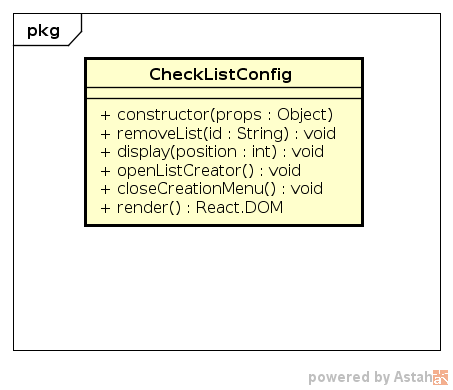
\includegraphics[width=0.6\textwidth]{img/single-CheckListConfig.png}
   \caption{{Diagramma per CheckListConfig in GuiCheckList}}
\end{figure}
\FloatBarrier
\textbf{Descrizione}\\
Componente React che rappresenta il menu principale per la creazione delle checklist. \\
\textbf{Metodi:} 
\begin{itemize}

\item +constructor(props : Object)
\\
Costruttore della sottoclasse di React.Component in cui è necessario chiamare super (props) ed è possibile inizializzare lo stato per i dati soggetti a cambiamento.

\item +removeList(id : String) : void  
\\
Metodo che rimuove una checklist dal database lato server

\item +render() : React.DOM 
\\
Metodo che esamina this.props e this.state e restituisce un singolo elemento React che può essere una rappresentazione di un componente DOM nativo o un altro componente composito.

\item +display(position : int): void
\\
Metodo che rende visibile la checklist con l'indice selezionato

\item +openListCreator(): void
\\
Metodo che gestisce l'apertura del menu di creazione di una nuova checklist
\item +closeCreationMenu(): void
\\
Metodo che gestisce la chiusura del menu di creazione di una nuova checklist

\end{itemize}

\textbf{Props:} 
\begin{itemize}

\item lists: 
\\
Array di oggetti, ciascuno dei quali rappresenta una checklist


\end{itemize} 


\textbf{Applicazioni}\\
Viene utilizzata per permettere la creazione, la modifica, l'eliminazione di checklists personalizzate 


\clearpage

\subsubsection{CheckListCreator}
\textbf{Componente:}  ListBubble::GuiCheckList\\
   \FloatBarrier
   \begin{figure}[ht]
   \centering
   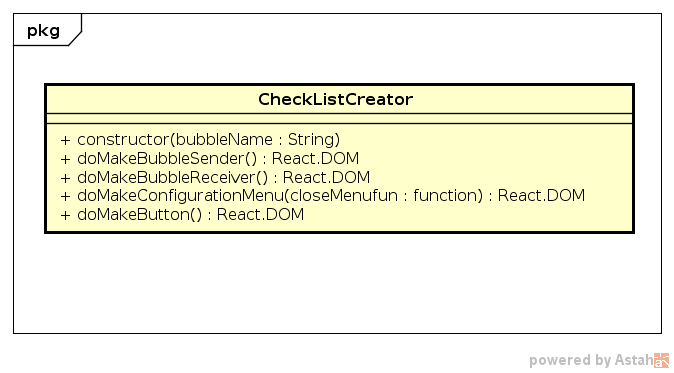
\includegraphics[width=0.6\textwidth]{img/single-CheckListCreator.png}
   \caption{{Diagramma per CheckListCreator in GuiCheckList}}
\end{figure}
\FloatBarrier
\textbf{Descrizione}\\
Istanziazione concreta della classe Monolith::UI::uiConstruction::BubbleCreator che viene utilizzata per inserire un componente grafico nell'area adibita al menu di configurazione delle bolle. A questo fine tutti i metodi tranne quello per creare menu di configurazione ritornano null.
\\
\textbf{Metodi:} 
\begin{itemize}
\item +constructor(bubbleName: String)
\item +doMakeBubbleSender() : React.DOM 
\item +doMakeBubbleReceiver() : React.DOM  
\item +doMakeConfigurationMenu() : React.DOM  
\\
Metodo che gestisce la creazione dell'area di configurazione della bolla.
\item +doMakeButton() : React.DOM  
\end{itemize} 


\textbf{Applicazioni}\\
Viene utilizzata per far funzionare un menu dedicato all'interno del sistema Monolith 


\clearpage

\subsubsection{CheckListEditing}
\textbf{Componente:}  ListBubble::GuiCheckList\\
   \FloatBarrier
   \begin{figure}[ht]
   \centering
   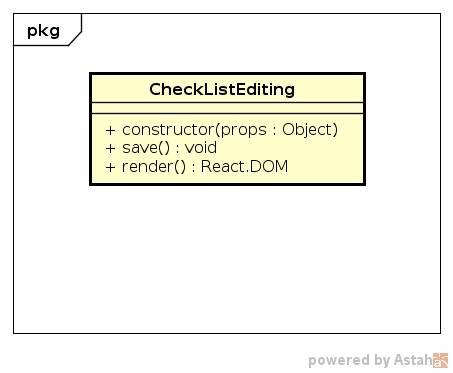
\includegraphics[width=0.6\textwidth]{img/single-CheckListEditing.png}
   \caption{{Diagramma per CheckListEditing in GuiCheckList}}
\end{figure}
\FloatBarrier
\textbf{Descrizione}\\
Componente React che gestisce la modifica delle checklists esistenti. \\
\textbf{Metodi:} 
\begin{itemize}

\item +constructor(props : Object) : React.Component 
\\
Costruttore della sottoclasse di React.Component in cui è necessario chiamare super (props) ed è possibile inizializzare lo stato per i dati soggetti a cambiamento.

\item +save() : void  
\\
Metodo che salva le modifiche alla checklist sul database

\item +render() : React.DOM 
\\
Metodo che esamina this.props e this.state e restituisce un singolo elemento React che può essere una rappresentazione di un componente DOM nativo o un altro componente composito.

\end{itemize}

\textbf{Props:} 
\begin{itemize}

\item title: 
\\
Stringa che rappresenta il titolo della checklist
\item ops:
\\
Array di stringhe che rappresenta gli elementi della checklist
\item hide:
\\
Booleano che determina se la lista sarà visibile o meno

\end{itemize} 


\textbf{Applicazioni}\\
Viene utilizzata per modificare le checklist esistenti 


\clearpage

\subsubsection{CheckListCreation}
\textbf{Componente:}  ListBubble::GuiCheckList\\
   \FloatBarrier
   \begin{figure}[ht]
   \centering
   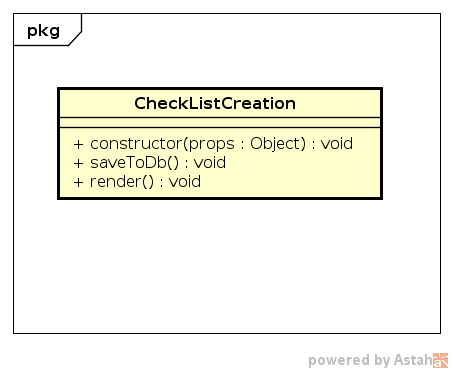
\includegraphics[width=0.6\textwidth]{img/single-CheckListCreation.png}
   \caption{{Diagramma per CheckListCreation in GuiCheckList}}
\end{figure}
\FloatBarrier
\textbf{Descrizione}\\
Componente React che gestisce la creazione di una nuova checklist \\
\textbf{Metodi:} 
\begin{itemize}

\item +constructor(props : Object)
\\
Costruttore della sottoclasse di React.Component in cui è necessario chiamare super (props) ed è possibile inizializzare lo stato per i dati soggetti a cambiamento.

\item +saveToDb() : void  
\\
Metodo che salva la checklist creata sul database

\item +render() : React.DOM 
\\
Metodo che esamina this.props e this.state e restituisce un singolo elemento React che può essere una rappresentazione di un componente DOM nativo o un altro componente composito.

\end{itemize}

\textbf{Props:} 
\begin{itemize}
\item closeMenu(): 
\\
Funzione che permette al componente di cancellarsi. Viene utilizzato in caso di esito positivo dell'invio.


\end{itemize} 


\textbf{Applicazioni}\\
Viene utilizzata per la creazione delle nuove checklists all'interno del menu dedicato 


\clearpage

\subsubsection{ListBubble}
\textbf{Componente:}  ListBubble::GuiList\\
   \FloatBarrier
   \begin{figure}[ht]
   \centering
   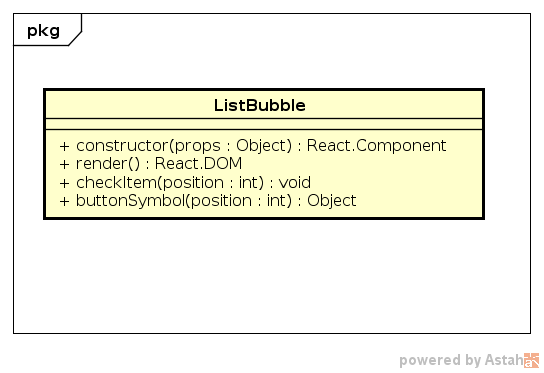
\includegraphics[width=0.6\textwidth]{img/single-ListBubble.png}
   \caption{{Diagramma per ListBubble in GuiList}}
\end{figure}
\FloatBarrier
\textbf{Descrizione}\\
Componente React che rappresenta l'interfaccia grafica di una ListBubble
\\
\textbf{Metodi:} 
\begin{itemize}
\item +constructor(props : Object) : React.Component 
\\
Costruttore della sottoclasse di React.Component in cui è necessario chiamare super (props) ed è possibile inizializzare lo stato per i dati soggetti a cambiamento.

\item +render() : React.DOM 
\\
Metodo che esamina this.props e this.state e restituisce elemento CheckBoxList 

\item +checkItem(position : int) : void 
\\
Metodo che riporta le spunte effettuate sul database lato server

\item +buttonSymbol(position:int): Object
\\
Metodo utilizzato dal render per determinare il comportamento dei pulsanti in caso il loro item corrispondente sia stato spuntato o meno. Nello specifico ritorna un oggetto che contiene il simbolo da visualizzare nel pulsante e un booleano che descrive lo stato di abilitazione del pulsante.

\end{itemize}

\textbf{Props:} 
\begin{itemize}
\item title: 
\\
Stringa che rappresenta il titolo della lista 
\item ops: 
\\
Array di oggetti formati da:
\begin{itemize}
\item item:String
\\
Rappresenta il testo dell'elemento della lista
\item check:boolean
\\
Rappresenta se l'item è stato spuntato o meno
\item id:int
\\
Identificativo numerico
\end{itemize}


\end{itemize} 


\textbf{Applicazioni}\\
Viene utilizzata per rappresentare graficamente la bolla Lista.
Viene istanziata automaticamente dal meccanismo di BubbleCreator nel pacchetto uiConstruction. 


\clearpage

\subsubsection{ListCreator}
\textbf{Componente:}  ListBubble::GuiList\\
   \FloatBarrier
   \begin{figure}[ht]
   \centering
   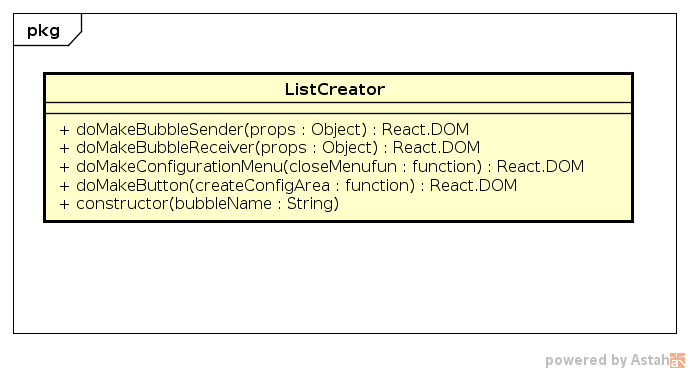
\includegraphics[width=0.6\textwidth]{img/single-ListCreator.png}
   \caption{{Diagramma per ListCreator in GuiList}}
\end{figure}
\FloatBarrier
\textbf{Descrizione}\\
Istanziazione concreta della classe Monolith::UI::uiConstruction::BubbleCreator che gestisce la creazione della singola istanza di bolla lista, della singola istanza di menù di configurazione della bolla e della singola istanza di pulsante tramite l'utilizzo della classe Monolith::UI::uiConstruction::BubbleDiscriminator.
\\
\textbf{Metodi:} 
\begin{itemize}
\item +constructor(bubbleName: String)
\item +doMakeBubbleSender(props: Object) : React.DOM 
\\
Metodo che gestisce la creazione della bolla vista dal mittente.
\item +doMakeBubbleReceiver(props: Object) : React.DOM 
\\
Metodo che gestisce la creazione della bolla vista dal ricevente.
\item +doMakeConfigurationMenu(closeMenufun: Function) : React.DOM  
\\
Metodo che gestisce la creazione dell'area di configurazione della bolla.
\item +doMakeButton(createConfigArea: Function) : React.DOM 
\\
Metodo che gestisce la creazione della singola istanza di pulsante da inserire nel menu iniziale di creazione. Viene lasciata l'implementazione della super classe.
\end{itemize} 


\textbf{Applicazioni}\\
Viene utilizzata per la creazione della singola istanza di bolla lista, della singola istanza di menù di configurazione della bolla e della singola istanza di pulsante 


\clearpage

\subsubsection{ListBubbleConfig}
\textbf{Componente:}  ListBubble::GuiList\\
   \FloatBarrier
   \begin{figure}[ht]
   \centering
   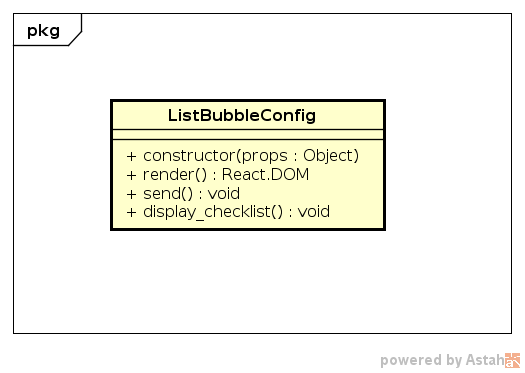
\includegraphics[width=0.6\textwidth]{img/single-ListBubbleConfig.png}
   \caption{{Diagramma per ListBubbleConfig in GuiList}}
\end{figure}
\FloatBarrier
\textbf{Descrizione}\\
Componente React che rappresenta il menù per la costruzione di una bolla Lista.
\\
\textbf{Metodi:} 
\begin{itemize}
\item +constructor(props : Object) : React.Component 
\\
Costruttore della sottoclasse di React.Component in cui è necessario chiamare super (props) ed è possibile inizializzare lo stato per i dati soggetti a cambiamento.

\item +display\_checklist() : void 
\\
Metodo che attiva o disattiva la visualizzazione della checklist

\item +send() : void 
\\
Salva i dati raccolti nel database

\item +render() : React.DOM
\\
Metodo che esamina this.props e this.state, costruisce un array di opzioni modificabili e restituisce l'interfaccia grafica per il menù di creazione.
\end{itemize}

\textbf{Props:} 
\begin{itemize}
\item closeMenu(): 
\\
Funzione che permette al componente di cancellarsi. Viene utilizzato in caso di esito positivo dell'invio.

\end{itemize} 


\textbf{Applicazioni}\\
Viene utilizzato per rappresentare il menù di configurazione della bolla Lista. 


\clearpage

\subsubsection{ListCheckListNavigation}
\textbf{Componente:}  ListBubble::GuiList\\
   \FloatBarrier
   \begin{figure}[ht]
   \centering
   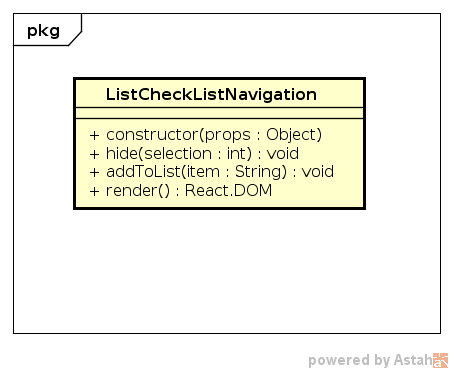
\includegraphics[width=0.6\textwidth]{img/single-ListCheckListNavigation.png}
   \caption{{Diagramma per ListCheckListNavigation in GuiList}}
\end{figure}
\FloatBarrier
\textbf{Descrizione}\\
Componente React che permette la visualizzazione delle checklists e l'aggiunta dei loro elementi alla lista.  \\
\textbf{Metodi:} 
\begin{itemize}

\item +constructor(props : Object)
\\
Costruttore della sottoclasse di React.Component in cui è necessario chiamare super (props) ed è possibile inizializzare lo stato per i dati soggetti a cambiamento.

\item +hide(selection : int) : void  
\\
Metodo che attiva o disattiva la visualizzazione della lista selezionata.

\item +addToList(item: String) : void
\\
Metodo che esegue props.add

\end{itemize}

\textbf{Props:} 
\begin{itemize}

\item lists: 
\\
Array di oggetti, ciascuno dei quali rappresenta una lista formata da:
\begin{itemize}
\item title: String
\item ops: Array of Strings

\end{itemize}
\item add(item: String)
\\
Metodo del genitore per aggiungere un elemento alla lista in costruzione in un ListBubbleConfig

\end{itemize} 


\textbf{Applicazioni}\\
Viene utilizzata per visualizzare le checklist durante la creazione delle liste e per aggiungere propri elementi alle liste 


\clearpage

\subsubsection{ListBubbleCreationButton}
\textbf{Componente:}  ListBubble::GuiList\\
   \FloatBarrier
   \begin{figure}[ht]
   \centering
   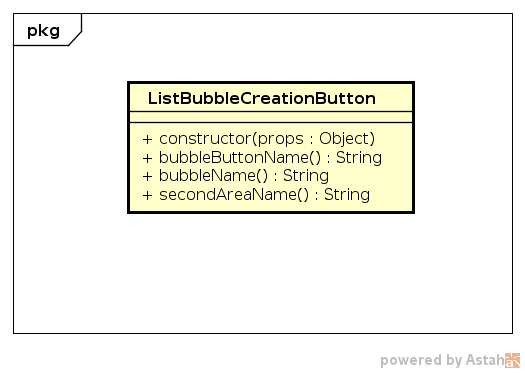
\includegraphics[width=0.6\textwidth]{img/single-ListBubbleCreationButton.png}
   \caption{{Diagramma per ListBubbleCreationButton in GuiList}}
\end{figure}
\FloatBarrier
\textbf{Descrizione}\\
Componente React che rappresenta il pulsante per creare una bolla Lista. Inoltre viene aggiunto un pulsante secondario per accedere al menu di creazione delle checklist.
\\
\textbf{Metodi:} 
\begin{itemize}
\item +constructor(props : Object)  
\\
Costruttore della sottoclasse di React.Component in cui è necessario chiamare super (props) ed è possibile inizializzare lo stato per i dati soggetti a cambiamento. Le props vengono usate solo dalla super classe.

\item +bubbleButtonName() : String 
\\
Metodo che ritorna il nome presente sul pulsante.

\item +bubbleName() : String 
\\
Metodo che ritorna il nome identificativo della bolla .

\item +secondAreaName() : String
\\
Metodo che ritorna il nome del componente grafico da costruire in risposta alla pressione del secondo pulsante

\end{itemize} 


\textbf{Applicazioni}\\
Viene utilizzato per rappresentare il pulsante per la creazione di una bolla Lista. 


\clearpage

\subsubsection{PollBubble}
\textbf{Componente:}  PollBubble\\
   \FloatBarrier
   \begin{figure}[ht]
   \centering
   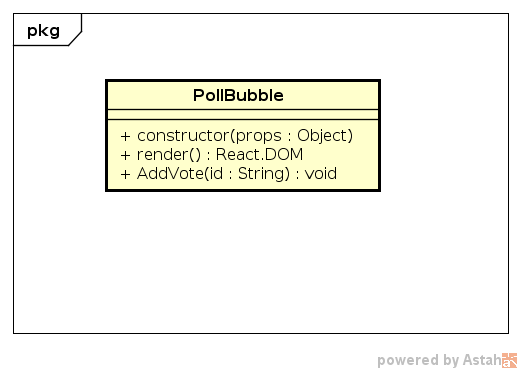
\includegraphics[width=0.6\textwidth]{img/single-PollBubble.png}
   \caption{{Diagramma per PollBubble in PollBubble}}
\end{figure}
\FloatBarrier
\textbf{Descrizione}\\
Componente React che rappresenta l'interfaccia grafica di una PollBubble
\\
\textbf{Metodi:} 
\begin{itemize}
\item +constructor(props : Object) : React.Component 
\\
Costruttore della sottoclasse di React.Component in cui è necessario chiamare super (props) ed è possibile inizializzare lo stato per i dati soggetti a cambiamento.

\item +render() : React.DOM 
\\
Metodo che esamina this.props e this.state e restituisce una lista di PushButton per votare il sondaggio. 

\item +addVoto(id : String) : void \\
Metodo che da un voto all'opzione selezionata. Permette di votare una sola volta.

\end{itemize}

\textbf{Props:} 
\begin{itemize}
\item title: 
\\
Stringa che rappresenta il titolo del sondaggio
\item options: 
\\
Array di oggetti formati da un id numerico, una stringa e un numero che rappresenta il numero di voti per quell'opzione.
\item \_id:
\\
id della bolla nel database
\item voted
\\
Array degli id degli utenti che hanno votato
\end{itemize} 


\textbf{Applicazioni}\\
Viene utilizzata per rappresentare graficamente la bolla Sondaggio. 


\clearpage

\subsubsection{PollCreator}
\textbf{Componente:}  PollBubble\\
   \FloatBarrier
   \begin{figure}[ht]
   \centering
   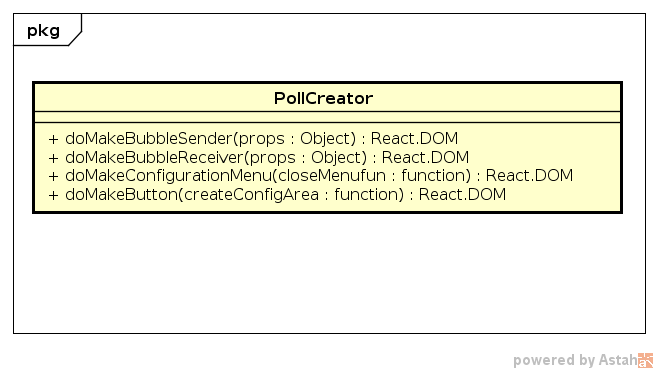
\includegraphics[width=0.6\textwidth]{img/single-PollCreator.png}
   \caption{{Diagramma per PollCreator in PollBubble}}
\end{figure}
\FloatBarrier
\textbf{Descrizione}\\
Istanziazione concreta della classe Monolith::UI::uiConstruction::BubbleCreator che gestisce la creazione della singola istanza di bolla sondaggio, della singola istanza di menù di configurazione della bolla e della singola istanza di pulsante tramite l'utilizzo della classe Monolith::UI::Bubbles::BubbleDiscriminator.
\\
\textbf{Metodi:} 
\begin{itemize}
\item +doMakeBubbleSender() : SurveyBubble 
\\
Metodo che gestisce la creazione della bolla vista dal mittente.
\item +doMakeBubbleReceiver() : SurveyBubble 
\\
Metodo che gestisce la creazione della bolla vista dal ricevente.
\item +doMakeConfigurationMenu() : SurveyBubbleConfig 
\\
Metodo che gestisce la creazione dell'area di configurazione della bolla.
\item +doMakeButton() : SurveyBubbleCreationButton 
\\
Metodo che gestisce la creazione della singola istanza di pulsante da inserire nel menu iniziale di creazione. Viene lasciata l'implementazione della super classe.
\end{itemize} 


\textbf{Applicazioni}\\
Viene utilizzata per gestire la creazione della singola istanza di bolla sondaggio, della singola istanza di menù di configurazione della bolla e della singola istanza di pulsante. 


\clearpage

\subsubsection{PollBubbleConfig}
\textbf{Componente:}  PollBubble\\
   \FloatBarrier
   \begin{figure}[ht]
   \centering
   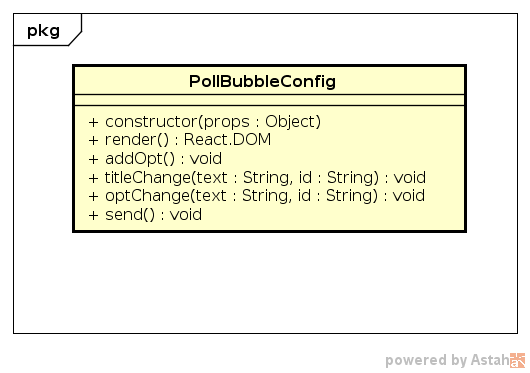
\includegraphics[width=0.6\textwidth]{img/single-PollBubbleConfig.png}
   \caption{{Diagramma per PollBubbleConfig in PollBubble}}
\end{figure}
\FloatBarrier
\textbf{Descrizione}\\
Componente React che rappresenta il menù per la costruzione di una bolla Sondaggio.
\\
\textbf{Metodi:} 
\begin{itemize}
\item +constructor(props : Object) : React.Component 
\\
Costruttore della sottoclasse di React.Component in cui è necessario chiamare super (props) ed è possibile inizializzare lo stato per i dati soggetti a cambiamento.

\item +addOpt() : void 
\\
Aggiunge un campo opzione in più ad ogni click sul tasto apposito.

\item +titleChange() : void 
\\
Salva il titolo che viene dato alla Lista.

\item +optChange() : void 
\\
Salva i valori che vengono dati ad ogni opzione.

\item +send() : void 
\\
Salva i dati raccolti e li passa al "padre".

\item +render() : React.DOM \\
Metodo che esamina this.props e this.state, costruisce un array di opzioni modificabili e restituisce l'interfaccia grafica per il menù di creazione.
\end{itemize}

\textbf{Props:} 
\begin{itemize}
\item closeMenu(): 
\\
Funzione che permette al componente di cancellarsi. Viene utilizzato in caso di esito positivo dell'invio.


\end{itemize} 


\textbf{Applicazioni}\\
Viene utilizzato per rappresentare il menù di configurazione della bolla Sondaggio. 


\clearpage

\subsubsection{PollBubbleCreationButton}
\textbf{Componente:}  PollBubble\\
   \FloatBarrier
   \begin{figure}[ht]
   \centering
   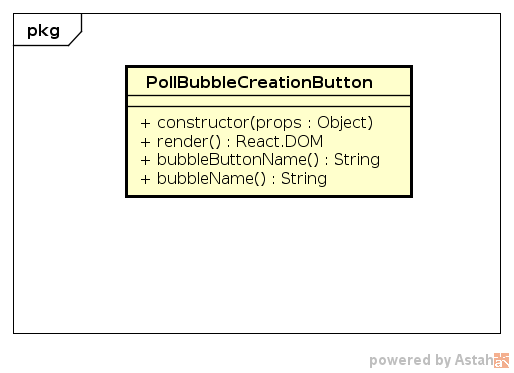
\includegraphics[width=0.6\textwidth]{img/single-PollBubbleCreationButton.png}
   \caption{{Diagramma per PollBubbleCreationButton in PollBubble}}
\end{figure}
\FloatBarrier
\textbf{Descrizione}\\
Componente React che rappresenta il pulsante per creare una bolla Sondaggio.
\\
\textbf{Metodi:} 
\begin{itemize}
\item +constructor(props : Object) : React.Component 
\\
Costruttore della sottoclasse di React.Component in cui è necessario chiamare super (props) ed è possibile inizializzare lo stato per i dati soggetti a cambiamento.

\item +bubbleButtonName() : String 
\\
Metodo che ritorna il nome presente sul pulsante.

\item +bubbleName() : String 
\\
Metodo che ritorna il nome identificativo della bolla .

\end{itemize}

\textbf{Props:} 
Non sono presenti props utilizzate direttamente. Vedere la superclasse AbsButton 


\textbf{Applicazioni}\\
Viene utilizzato per rappresentare il pulsante per la creazione di una bolla Sondaggio. 


\clearpage

\subsubsection{RandBubble}
\textbf{Componente:}  RandomBubble\\
   \FloatBarrier
   \begin{figure}[ht]
   \centering
   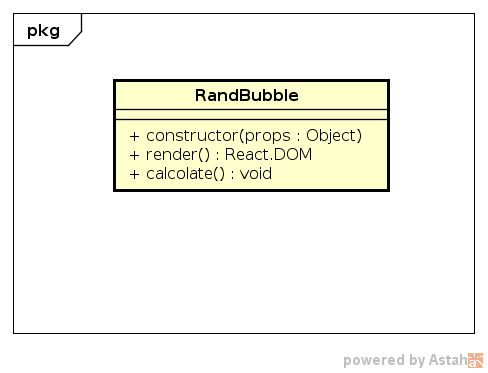
\includegraphics[width=0.6\textwidth]{img/single-RandBubble.png}
   \caption{{Diagramma per RandBubble in RandomBubble}}
\end{figure}
\FloatBarrier
\textbf{Descrizione}\\
Componente React che rappresenta l'interfaccia grafica di una RandBubble
\\
\textbf{Metodi:} 
\begin{itemize}
\item +constructor(props : Object) : React.Component 
\\
Costruttore della sottoclasse di React.Component in cui è necessario chiamare super (props) ed è possibile inizializzare lo stato per i dati soggetti a cambiamento. 

\item +render() : React.DOM 
\\
Metodo che esamina this.props e this.state e restituisce il numero random calcolato. 

\item +calcolate() : void \\
Metodo che passa al "padre" il nuovo numero random estratto.
\end{itemize}

\textbf{Props:} 
\begin{itemize}
\item \_id: 
\\
id della bolla nel database
\item range: 
\\
Numero che rappresenta il massimo valore tra quelli estraibili
\item value
\\
Numero che rappresenta il valore casuale estratto

\end{itemize} 


\textbf{Applicazioni}\\
Viene utilizzata per rappresentare graficamente la bolla Random. 


\clearpage

\subsubsection{RandCreator}
\textbf{Componente:}  RandomBubble\\
   \FloatBarrier
   \begin{figure}[ht]
   \centering
   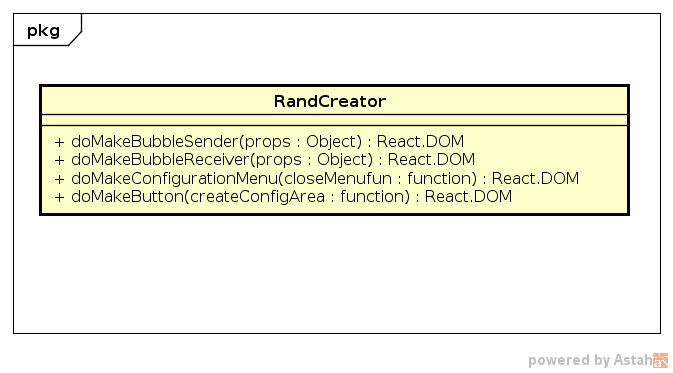
\includegraphics[width=0.6\textwidth]{img/single-RandCreator.png}
   \caption{{Diagramma per RandCreator in RandomBubble}}
\end{figure}
\FloatBarrier
\textbf{Descrizione}\\
Istanziazione concreta della classe Monolith::UI::uiConstruction::BubbleCreator che gestisce la creazione della singola istanza di bolla estrazione di numero casuale, della singola istanza di menù di configurazione della bolla e della singola istanza di pulsante tramite l'utilizzo della classe Monolith::UI::Bubbles::BubbleDiscriminator.
\\
\textbf{Metodi:} 
\begin{itemize}
\item +doMakeBubbleSender() : DiceBubble 
\\
Metodo che gestisce la creazione della bolla vista dal mittente.
\item +doMakeBubbleReceiver() : DiceBubble 
\\
Metodo che gestisce la creazione della bolla vista dal ricevente.
\item +doMakeConfigurationMenu() : DiceBubbleConfig 
\\
Metodo che gestisce la creazione dell'area di configurazione della bolla.
\item +doMakeButton() : DiceBubbleCreationButton 
\\
Metodo che gestisce la creazione della singola istanza di pulsante da inserire nel menu iniziale di creazione. Viene lasciata l'implementazione della super classe.
\end{itemize} 


\textbf{Applicazioni}\\
Viene utilizzata per gestire la creazione della singola istanza di bolla estrazione di numero casuale, della singola istanza di menù di configurazione della bolla e della singola istanza di pulsante. 


\clearpage

\subsubsection{RandBubbleConfig}
\textbf{Componente:}  RandomBubble\\
   \FloatBarrier
   \begin{figure}[ht]
   \centering
   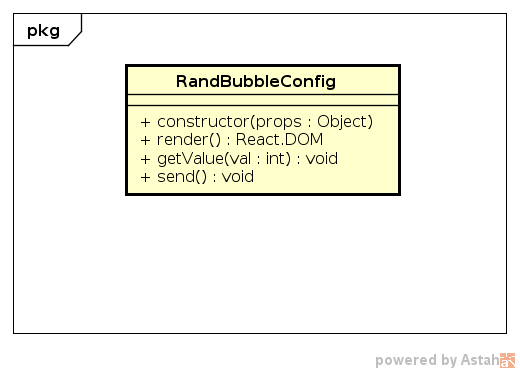
\includegraphics[width=0.6\textwidth]{img/single-RandBubbleConfig.png}
   \caption{{Diagramma per RandBubbleConfig in RandomBubble}}
\end{figure}
\FloatBarrier
\textbf{Descrizione}\\
Componente React che rappresenta il menù per la costruzione di una bolla di conversione valuta.
\\
\textbf{Metodi:} 
\begin{itemize}
\item +constructor(props : Object) : React.Component 
\\
Costruttore della sottoclasse di React.Component in cui è necessario chiamare super (props) ed è possibile inizializzare lo stato per i dati soggetti a cambiamento.

\item +getValue(val: String) : void 
\\
Salva il numero di facce del dado.

\item +send() : void 
\\
Salva i dati raccolti e li passa al "padre".

\item +render() : React.DOM \\
Metodo che esamina this.props e this.state e restituisce l'interfaccia grafica per il menù di creazione.
\end{itemize}

\textbf{Props:} 
\begin{itemize}
\item closeMenu(): 
\\
Funzione che permette al componente di cancellarsi. Viene utilizzato in caso di esito positivo dell'invio.
\end{itemize} 


\textbf{Applicazioni}\\
Viene utilizzato per rappresentare il menù di configurazione della bolla di lancio casuale di dadi. 


\clearpage

\subsubsection{RandBubbleCreationButton}
\textbf{Componente:}  RandomBubble\\
   \FloatBarrier
   \begin{figure}[ht]
   \centering
   \includegraphics[width=0.6\textwidth]{img/single-RandBubbleCreationButton.png}
   \caption{{Diagramma per RandBubbleCreationButton in RandomBubble}}
\end{figure}
\FloatBarrier
\textbf{Descrizione}\\
Componente React che rappresenta il pulsante per creare una bolla di lancio casuale di dadi.
\\
\textbf{Metodi:} 
\begin{itemize}
\item +constructor(props : Object) : React.Component 
\\
Costruttore della sottoclasse di React.Component in cui è necessario chiamare super (props) ed è possibile inizializzare lo stato per i dati soggetti a cambiamento.

\item +bubbleButtonName() : String 
\\
Metodo che ritorna il nome presente sul pulsante.

\item +bubbleName() : String 
\\
Metodo che ritorna il nome identificativo della bolla .

\end{itemize}

\textbf{Props:} 
Non sono presenti props utilizzate direttamente. Vedere la superclasse AbsButton 


\textbf{Applicazioni}\\
Viene utilizzato per rappresentare il pulsante per la creazione di una bolla di lancio casuale di dadi. 


